% Created by tikzDevice version 0.7.0 on 2014-07-01 19:29:10
% !TEX encoding = UTF-8 Unicode
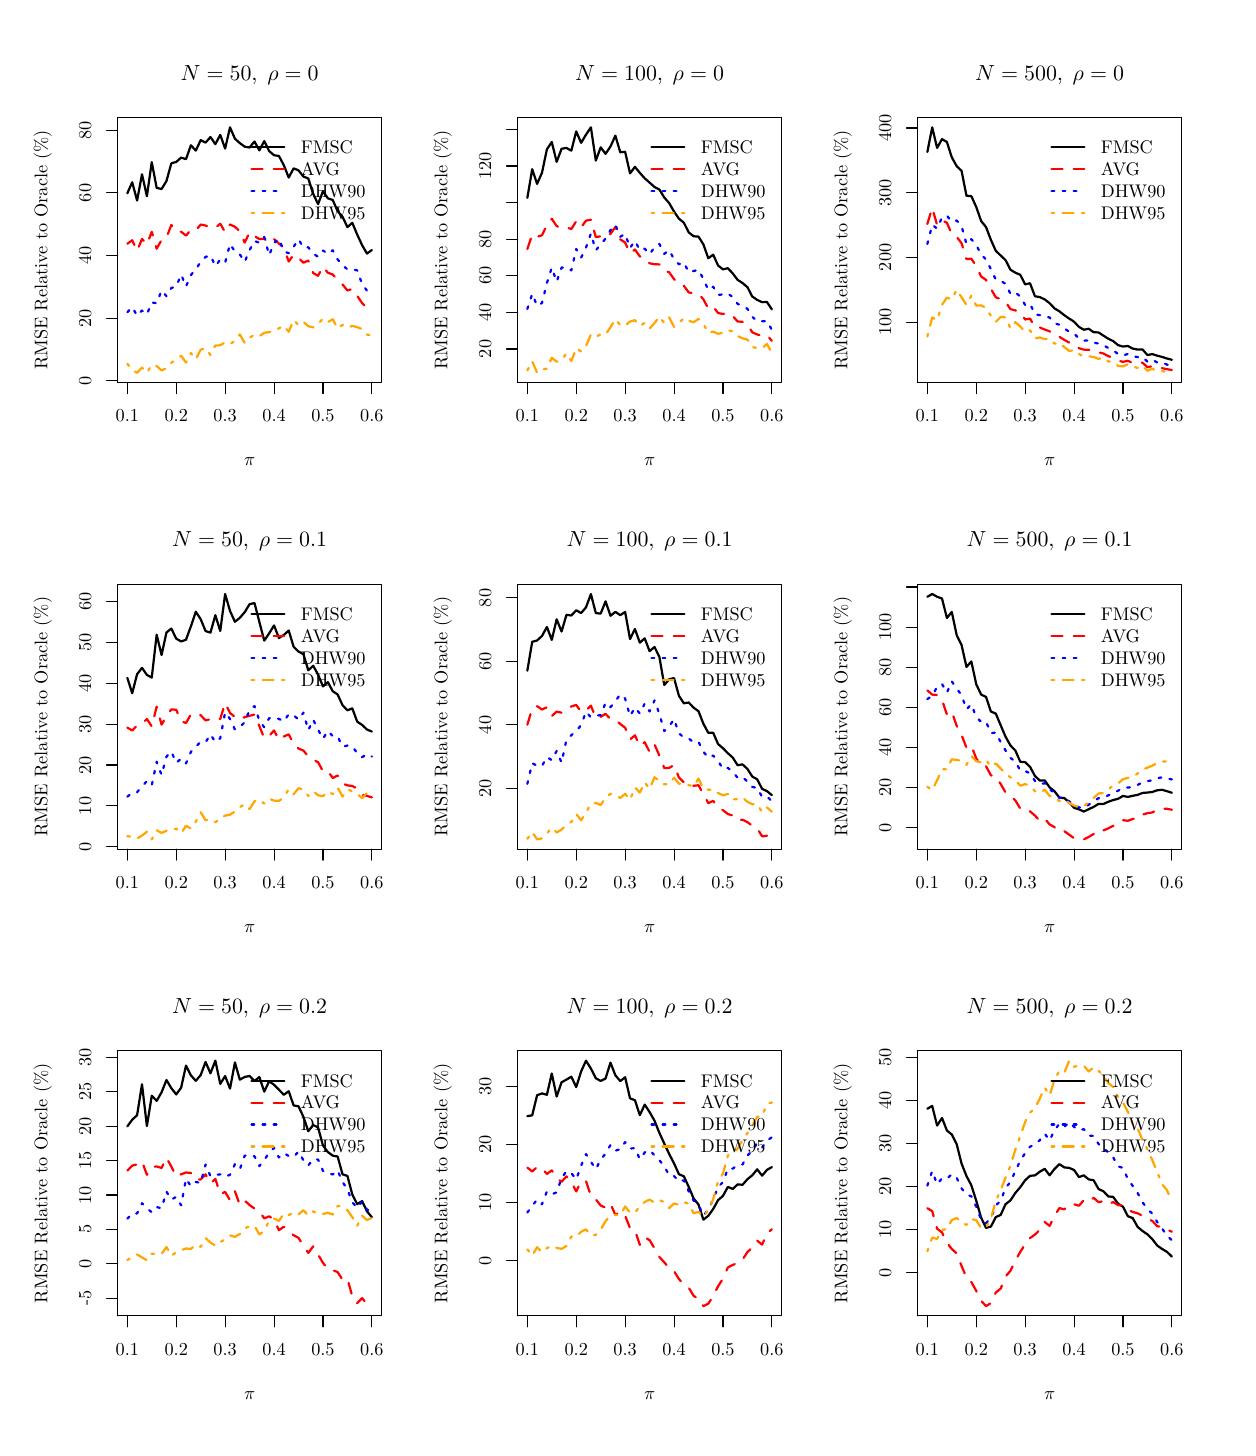
\begin{tikzpicture}[x=1pt,y=1pt]
\definecolor[named]{fillColor}{rgb}{1.00,1.00,1.00}
\path[use as bounding box,fill=fillColor,fill opacity=0.00] (0,0) rectangle (433.62,505.89);
\begin{scope}
\path[clip] ( 32.47,377.65) rectangle (127.91,473.42);
\definecolor[named]{drawColor}{rgb}{0.00,0.00,0.00}

\path[draw=drawColor,line width= 0.8pt,line join=round,line cap=round] ( 36.01,446.04) --
	( 37.77,450.01) --
	( 39.54,443.42) --
	( 41.31,452.91) --
	( 43.08,444.98) --
	( 44.84,457.29) --
	( 46.61,447.99) --
	( 48.38,447.58) --
	( 50.15,450.47) --
	( 51.91,456.88) --
	( 53.68,457.37) --
	( 55.45,458.94) --
	( 57.21,458.37) --
	( 58.98,463.40) --
	( 60.75,461.47) --
	( 62.52,465.25) --
	( 64.28,464.34) --
	( 66.05,466.38) --
	( 67.82,463.79) --
	( 69.59,467.15) --
	( 71.35,462.19) --
	( 73.12,469.87) --
	( 74.89,465.76) --
	( 76.66,464.17) --
	( 78.42,462.89) --
	( 80.19,462.59) --
	( 81.96,464.75) --
	( 83.72,461.54) --
	( 85.49,464.90) --
	( 87.26,461.28) --
	( 89.03,459.79) --
	( 90.79,459.53) --
	( 92.56,456.17) --
	( 94.33,451.73) --
	( 96.10,455.04) --
	( 97.86,454.33) --
	( 99.63,452.09) --
	(101.40,451.38) --
	(103.17,445.85) --
	(104.93,442.12) --
	(106.70,446.78) --
	(108.47,444.23) --
	(110.23,443.64) --
	(112.00,439.56) --
	(113.77,437.56) --
	(115.54,433.81) --
	(117.30,435.37) --
	(119.07,431.13) --
	(120.84,427.30) --
	(122.61,424.25) --
	(124.37,425.53);
\end{scope}
\begin{scope}
\path[clip] (  0.00,  0.00) rectangle (433.62,505.89);
\definecolor[named]{drawColor}{rgb}{0.00,0.00,0.00}

\path[draw=drawColor,line width= 0.4pt,line join=round,line cap=round] ( 36.01,377.65) -- (124.37,377.65);

\path[draw=drawColor,line width= 0.4pt,line join=round,line cap=round] ( 36.01,377.65) -- ( 36.01,373.69);

\path[draw=drawColor,line width= 0.4pt,line join=round,line cap=round] ( 53.68,377.65) -- ( 53.68,373.69);

\path[draw=drawColor,line width= 0.4pt,line join=round,line cap=round] ( 71.35,377.65) -- ( 71.35,373.69);

\path[draw=drawColor,line width= 0.4pt,line join=round,line cap=round] ( 89.03,377.65) -- ( 89.03,373.69);

\path[draw=drawColor,line width= 0.4pt,line join=round,line cap=round] (106.70,377.65) -- (106.70,373.69);

\path[draw=drawColor,line width= 0.4pt,line join=round,line cap=round] (124.37,377.65) -- (124.37,373.69);

\node[text=drawColor,anchor=base,inner sep=0pt, outer sep=0pt, scale=  0.66] at ( 36.01,363.40) {0.1};

\node[text=drawColor,anchor=base,inner sep=0pt, outer sep=0pt, scale=  0.66] at ( 53.68,363.40) {0.2};

\node[text=drawColor,anchor=base,inner sep=0pt, outer sep=0pt, scale=  0.66] at ( 71.35,363.40) {0.3};

\node[text=drawColor,anchor=base,inner sep=0pt, outer sep=0pt, scale=  0.66] at ( 89.03,363.40) {0.4};

\node[text=drawColor,anchor=base,inner sep=0pt, outer sep=0pt, scale=  0.66] at (106.70,363.40) {0.5};

\node[text=drawColor,anchor=base,inner sep=0pt, outer sep=0pt, scale=  0.66] at (124.37,363.40) {0.6};

\path[draw=drawColor,line width= 0.4pt,line join=round,line cap=round] ( 32.47,378.33) -- ( 32.47,468.79);

\path[draw=drawColor,line width= 0.4pt,line join=round,line cap=round] ( 32.47,378.33) -- ( 28.51,378.33);

\path[draw=drawColor,line width= 0.4pt,line join=round,line cap=round] ( 32.47,400.95) -- ( 28.51,400.95);

\path[draw=drawColor,line width= 0.4pt,line join=round,line cap=round] ( 32.47,423.56) -- ( 28.51,423.56);

\path[draw=drawColor,line width= 0.4pt,line join=round,line cap=round] ( 32.47,446.18) -- ( 28.51,446.18);

\path[draw=drawColor,line width= 0.4pt,line join=round,line cap=round] ( 32.47,468.79) -- ( 28.51,468.79);

\node[text=drawColor,rotate= 90.00,anchor=base,inner sep=0pt, outer sep=0pt, scale=  0.66] at ( 22.97,378.33) {0};

\node[text=drawColor,rotate= 90.00,anchor=base,inner sep=0pt, outer sep=0pt, scale=  0.66] at ( 22.97,400.95) {20};

\node[text=drawColor,rotate= 90.00,anchor=base,inner sep=0pt, outer sep=0pt, scale=  0.66] at ( 22.97,423.56) {40};

\node[text=drawColor,rotate= 90.00,anchor=base,inner sep=0pt, outer sep=0pt, scale=  0.66] at ( 22.97,446.18) {60};

\node[text=drawColor,rotate= 90.00,anchor=base,inner sep=0pt, outer sep=0pt, scale=  0.66] at ( 22.97,468.79) {80};

\path[draw=drawColor,line width= 0.4pt,line join=round,line cap=round] ( 32.47,377.65) --
	(127.91,377.65) --
	(127.91,473.42) --
	( 32.47,473.42) --
	( 32.47,377.65);
\end{scope}
\begin{scope}
\path[clip] (  0.00,337.26) rectangle (144.54,505.89);
\definecolor[named]{drawColor}{rgb}{0.00,0.00,0.00}

\node[text=drawColor,anchor=base,inner sep=0pt, outer sep=0pt, scale=  0.79] at ( 80.19,486.92) {\bfseries $N=50, \;\rho=0$};

\node[text=drawColor,anchor=base,inner sep=0pt, outer sep=0pt, scale=  0.66] at ( 80.19,347.56) {$\pi$};

\node[text=drawColor,rotate= 90.00,anchor=base,inner sep=0pt, outer sep=0pt, scale=  0.66] at (  7.13,425.53) {RMSE Relative to Oracle (\%)};
\end{scope}
\begin{scope}
\path[clip] ( 32.47,377.65) rectangle (127.91,473.42);
\definecolor[named]{drawColor}{rgb}{1.00,0.00,0.00}

\path[draw=drawColor,line width= 0.8pt,dash pattern=on 4pt off 4pt ,line join=round,line cap=round] ( 36.01,427.81) --
	( 37.77,429.06) --
	( 39.54,425.23) --
	( 41.31,429.56) --
	( 43.08,427.54) --
	( 44.84,432.11) --
	( 46.61,426.02) --
	( 48.38,429.17) --
	( 50.15,429.96) --
	( 51.91,434.61) --
	( 53.68,432.38) --
	( 55.45,432.14) --
	( 57.21,430.75) --
	( 58.98,432.82) --
	( 60.75,432.63) --
	( 62.52,434.74) --
	( 64.28,434.39) --
	( 66.05,433.70) --
	( 67.82,433.60) --
	( 69.59,435.06) --
	( 71.35,431.93) --
	( 73.12,434.76) --
	( 74.89,433.94) --
	( 76.66,432.32) --
	( 78.42,428.22) --
	( 80.19,431.93) --
	( 81.96,430.57) --
	( 83.72,429.50) --
	( 85.49,429.64) --
	( 87.26,428.02) --
	( 89.03,429.47) --
	( 90.79,427.88) --
	( 92.56,426.39) --
	( 94.33,421.38) --
	( 96.10,423.88) --
	( 97.86,422.71) --
	( 99.63,420.96) --
	(101.40,421.71) --
	(103.17,417.21) --
	(104.93,416.23) --
	(106.70,419.57) --
	(108.47,417.32) --
	(110.23,416.71) --
	(112.00,414.61) --
	(113.77,413.09) --
	(115.54,410.93) --
	(117.30,411.46) --
	(119.07,408.97) --
	(120.84,406.35) --
	(122.61,404.70) --
	(124.37,405.65);
\definecolor[named]{drawColor}{rgb}{0.00,0.00,1.00}

\path[draw=drawColor,line width= 0.8pt,dash pattern=on 1pt off 3pt ,line join=round,line cap=round] ( 36.01,403.05) --
	( 37.77,404.89) --
	( 39.54,401.81) --
	( 41.31,403.68) --
	( 43.08,402.29) --
	( 44.84,406.58) --
	( 46.61,406.33) --
	( 48.38,410.90) --
	( 50.15,408.87) --
	( 51.91,411.83) --
	( 53.68,412.36) --
	( 55.45,416.66) --
	( 57.21,412.36) --
	( 58.98,416.49) --
	( 60.75,418.67) --
	( 62.52,421.15) --
	( 64.28,423.06) --
	( 66.05,423.59) --
	( 67.82,419.71) --
	( 69.59,422.09) --
	( 71.35,420.98) --
	( 73.12,427.73) --
	( 74.89,424.99) --
	( 76.66,423.95) --
	( 78.42,421.24) --
	( 80.19,425.55) --
	( 81.96,428.80) --
	( 83.72,428.16) --
	( 85.49,430.27) --
	( 87.26,423.68) --
	( 89.03,428.10) --
	( 90.79,429.65) --
	( 92.56,425.08) --
	( 94.33,424.37) --
	( 96.10,426.69) --
	( 97.86,429.43) --
	( 99.63,426.47) --
	(101.40,426.51) --
	(103.17,424.22) --
	(104.93,423.09) --
	(106.70,425.38) --
	(108.47,424.17) --
	(110.23,425.44) --
	(112.00,422.13) --
	(113.77,420.11) --
	(115.54,418.51) --
	(117.30,418.61) --
	(119.07,418.17) --
	(120.84,413.28) --
	(122.61,410.85) --
	(124.37,412.71);
\definecolor[named]{drawColor}{rgb}{1.00,0.65,0.00}

\path[draw=drawColor,line width= 0.8pt,dash pattern=on 1pt off 3pt on 4pt off 3pt ,line join=round,line cap=round] ( 36.01,384.45) --
	( 37.77,382.14) --
	( 39.54,381.20) --
	( 41.31,383.07) --
	( 43.08,381.22) --
	( 44.84,384.04) --
	( 46.61,383.60) --
	( 48.38,382.04) --
	( 50.15,382.81) --
	( 51.91,384.80) --
	( 53.68,386.03) --
	( 55.45,387.33) --
	( 57.21,384.88) --
	( 58.98,388.28) --
	( 60.75,386.07) --
	( 62.52,389.54) --
	( 64.28,390.04) --
	( 66.05,387.63) --
	( 67.82,391.05) --
	( 69.59,391.11) --
	( 71.35,392.19) --
	( 73.12,391.54) --
	( 74.89,392.74) --
	( 76.66,395.05) --
	( 78.42,391.94) --
	( 80.19,393.85) --
	( 81.96,394.93) --
	( 83.72,394.38) --
	( 85.49,395.66) --
	( 87.26,395.85) --
	( 89.03,396.36) --
	( 90.79,397.25) --
	( 92.56,398.22) --
	( 94.33,395.98) --
	( 96.10,400.30) --
	( 97.86,398.39) --
	( 99.63,399.59) --
	(101.40,398.01) --
	(103.17,397.59) --
	(104.93,398.82) --
	(106.70,400.75) --
	(108.47,399.50) --
	(110.23,400.53) --
	(112.00,397.20) --
	(113.77,398.51) --
	(115.54,397.51) --
	(117.30,398.11) --
	(119.07,397.68) --
	(120.84,396.96) --
	(122.61,395.01) --
	(124.37,394.61);
\definecolor[named]{drawColor}{rgb}{0.00,0.00,0.00}

\path[draw=drawColor,line width= 0.8pt,line join=round,line cap=round] ( 80.89,462.63) -- ( 92.77,462.63);
\definecolor[named]{drawColor}{rgb}{1.00,0.00,0.00}

\path[draw=drawColor,line width= 0.8pt,dash pattern=on 4pt off 4pt ,line join=round,line cap=round] ( 80.89,454.71) -- ( 92.77,454.71);
\definecolor[named]{drawColor}{rgb}{0.00,0.00,1.00}

\path[draw=drawColor,line width= 0.8pt,dash pattern=on 1pt off 3pt ,line join=round,line cap=round] ( 80.89,446.79) -- ( 92.77,446.79);
\definecolor[named]{drawColor}{rgb}{1.00,0.65,0.00}

\path[draw=drawColor,line width= 0.8pt,dash pattern=on 1pt off 3pt on 4pt off 3pt ,line join=round,line cap=round] ( 80.89,438.87) -- ( 92.77,438.87);
\definecolor[named]{drawColor}{rgb}{0.00,0.00,0.00}

\node[text=drawColor,anchor=base west,inner sep=0pt, outer sep=0pt, scale=  0.66] at ( 98.71,460.35) {FMSC};

\node[text=drawColor,anchor=base west,inner sep=0pt, outer sep=0pt, scale=  0.66] at ( 98.71,452.43) {AVG};

\node[text=drawColor,anchor=base west,inner sep=0pt, outer sep=0pt, scale=  0.66] at ( 98.71,444.51) {DHW90};

\node[text=drawColor,anchor=base west,inner sep=0pt, outer sep=0pt, scale=  0.66] at ( 98.71,436.59) {DHW95};
\end{scope}
\begin{scope}
\path[clip] (177.01,377.65) rectangle (272.45,473.42);
\definecolor[named]{drawColor}{rgb}{0.00,0.00,0.00}

\path[draw=drawColor,line width= 0.8pt,line join=round,line cap=round] (180.55,444.38) --
	(182.31,454.74) --
	(184.08,449.44) --
	(185.85,453.47) --
	(187.62,461.92) --
	(189.38,464.57) --
	(191.15,457.39) --
	(192.92,462.14) --
	(194.69,462.42) --
	(196.45,461.43) --
	(198.22,468.41) --
	(199.99,464.26) --
	(201.75,467.24) --
	(203.52,469.87) --
	(205.29,457.86) --
	(207.06,462.64) --
	(208.82,460.29) --
	(210.59,462.93) --
	(212.36,466.86) --
	(214.13,460.87) --
	(215.89,461.03) --
	(217.66,453.24) --
	(219.43,455.60) --
	(221.20,453.43) --
	(222.96,451.45) --
	(224.73,449.91) --
	(226.50,448.31) --
	(228.26,447.41) --
	(230.03,444.51) --
	(231.80,442.49) --
	(233.57,439.42) --
	(235.33,436.88) --
	(237.10,435.41) --
	(238.87,431.91) --
	(240.64,430.51) --
	(242.40,430.38) --
	(244.17,427.56) --
	(245.94,422.58) --
	(247.71,423.84) --
	(249.47,419.97) --
	(251.24,418.53) --
	(253.01,418.97) --
	(254.77,417.08) --
	(256.54,414.75) --
	(258.31,413.62) --
	(260.08,412.11) --
	(261.84,408.71) --
	(263.61,407.52) --
	(265.38,406.70) --
	(267.15,406.74) --
	(268.91,404.09);
\end{scope}
\begin{scope}
\path[clip] (  0.00,  0.00) rectangle (433.62,505.89);
\definecolor[named]{drawColor}{rgb}{0.00,0.00,0.00}

\path[draw=drawColor,line width= 0.4pt,line join=round,line cap=round] (180.55,377.65) -- (268.91,377.65);

\path[draw=drawColor,line width= 0.4pt,line join=round,line cap=round] (180.55,377.65) -- (180.55,373.69);

\path[draw=drawColor,line width= 0.4pt,line join=round,line cap=round] (198.22,377.65) -- (198.22,373.69);

\path[draw=drawColor,line width= 0.4pt,line join=round,line cap=round] (215.89,377.65) -- (215.89,373.69);

\path[draw=drawColor,line width= 0.4pt,line join=round,line cap=round] (233.57,377.65) -- (233.57,373.69);

\path[draw=drawColor,line width= 0.4pt,line join=round,line cap=round] (251.24,377.65) -- (251.24,373.69);

\path[draw=drawColor,line width= 0.4pt,line join=round,line cap=round] (268.91,377.65) -- (268.91,373.69);

\node[text=drawColor,anchor=base,inner sep=0pt, outer sep=0pt, scale=  0.66] at (180.55,363.40) {0.1};

\node[text=drawColor,anchor=base,inner sep=0pt, outer sep=0pt, scale=  0.66] at (198.22,363.40) {0.2};

\node[text=drawColor,anchor=base,inner sep=0pt, outer sep=0pt, scale=  0.66] at (215.89,363.40) {0.3};

\node[text=drawColor,anchor=base,inner sep=0pt, outer sep=0pt, scale=  0.66] at (233.57,363.40) {0.4};

\node[text=drawColor,anchor=base,inner sep=0pt, outer sep=0pt, scale=  0.66] at (251.24,363.40) {0.5};

\node[text=drawColor,anchor=base,inner sep=0pt, outer sep=0pt, scale=  0.66] at (268.91,363.40) {0.6};

\path[draw=drawColor,line width= 0.4pt,line join=round,line cap=round] (177.01,389.78) -- (177.01,469.12);

\path[draw=drawColor,line width= 0.4pt,line join=round,line cap=round] (177.01,389.78) -- (173.05,389.78);

\path[draw=drawColor,line width= 0.4pt,line join=round,line cap=round] (177.01,403.00) -- (173.05,403.00);

\path[draw=drawColor,line width= 0.4pt,line join=round,line cap=round] (177.01,416.23) -- (173.05,416.23);

\path[draw=drawColor,line width= 0.4pt,line join=round,line cap=round] (177.01,429.45) -- (173.05,429.45);

\path[draw=drawColor,line width= 0.4pt,line join=round,line cap=round] (177.01,442.67) -- (173.05,442.67);

\path[draw=drawColor,line width= 0.4pt,line join=round,line cap=round] (177.01,455.90) -- (173.05,455.90);

\path[draw=drawColor,line width= 0.4pt,line join=round,line cap=round] (177.01,469.12) -- (173.05,469.12);

\node[text=drawColor,rotate= 90.00,anchor=base,inner sep=0pt, outer sep=0pt, scale=  0.66] at (167.51,389.78) {20};

\node[text=drawColor,rotate= 90.00,anchor=base,inner sep=0pt, outer sep=0pt, scale=  0.66] at (167.51,403.00) {40};

\node[text=drawColor,rotate= 90.00,anchor=base,inner sep=0pt, outer sep=0pt, scale=  0.66] at (167.51,416.23) {60};

\node[text=drawColor,rotate= 90.00,anchor=base,inner sep=0pt, outer sep=0pt, scale=  0.66] at (167.51,429.45) {80};

\node[text=drawColor,rotate= 90.00,anchor=base,inner sep=0pt, outer sep=0pt, scale=  0.66] at (167.51,455.90) {120};

\path[draw=drawColor,line width= 0.4pt,line join=round,line cap=round] (177.01,377.65) --
	(272.45,377.65) --
	(272.45,473.42) --
	(177.01,473.42) --
	(177.01,377.65);
\end{scope}
\begin{scope}
\path[clip] (144.54,337.26) rectangle (289.08,505.89);
\definecolor[named]{drawColor}{rgb}{0.00,0.00,0.00}

\node[text=drawColor,anchor=base,inner sep=0pt, outer sep=0pt, scale=  0.79] at (224.73,486.92) {\bfseries $N=100, \;\rho=0$};

\node[text=drawColor,anchor=base,inner sep=0pt, outer sep=0pt, scale=  0.66] at (224.73,347.56) {$\pi$};

\node[text=drawColor,rotate= 90.00,anchor=base,inner sep=0pt, outer sep=0pt, scale=  0.66] at (151.67,425.53) {RMSE Relative to Oracle (\%)};
\end{scope}
\begin{scope}
\path[clip] (177.01,377.65) rectangle (272.45,473.42);
\definecolor[named]{drawColor}{rgb}{1.00,0.00,0.00}

\path[draw=drawColor,line width= 0.8pt,dash pattern=on 4pt off 4pt ,line join=round,line cap=round] (180.55,425.91) --
	(182.31,431.18) --
	(184.08,430.36) --
	(185.85,430.86) --
	(187.62,434.61) --
	(189.38,436.83) --
	(191.15,434.17) --
	(192.92,433.59) --
	(194.69,433.74) --
	(196.45,433.12) --
	(198.22,435.94) --
	(199.99,433.77) --
	(201.75,436.16) --
	(203.52,436.50) --
	(205.29,430.22) --
	(207.06,430.48) --
	(208.82,430.10) --
	(210.59,431.40) --
	(212.36,433.83) --
	(214.13,429.38) --
	(215.89,428.25) --
	(217.66,424.31) --
	(219.43,425.73) --
	(221.20,423.22) --
	(222.96,422.83) --
	(224.73,420.75) --
	(226.50,420.39) --
	(228.26,420.34) --
	(230.03,418.12) --
	(231.80,417.49) --
	(233.57,415.01) --
	(235.33,413.23) --
	(237.10,412.61) --
	(238.87,410.22) --
	(240.64,409.88) --
	(242.40,409.70) --
	(244.17,407.73) --
	(245.94,404.40) --
	(247.71,405.09) --
	(249.47,402.77) --
	(251.24,402.44) --
	(253.01,402.76) --
	(254.77,401.70) --
	(256.54,399.71) --
	(258.31,399.60) --
	(260.08,398.61) --
	(261.84,395.80) --
	(263.61,395.03) --
	(265.38,394.55) --
	(267.15,394.75) --
	(268.91,392.71);
\definecolor[named]{drawColor}{rgb}{0.00,0.00,1.00}

\path[draw=drawColor,line width= 0.8pt,dash pattern=on 1pt off 3pt ,line join=round,line cap=round] (180.55,404.24) --
	(182.31,409.69) --
	(184.08,405.35) --
	(185.85,406.40) --
	(187.62,413.60) --
	(189.38,419.16) --
	(191.15,414.07) --
	(192.92,419.19) --
	(194.69,419.28) --
	(196.45,418.16) --
	(198.22,425.92) --
	(199.99,422.77) --
	(201.75,426.47) --
	(203.52,431.47) --
	(205.29,425.42) --
	(207.06,427.59) --
	(208.82,429.66) --
	(210.59,432.74) --
	(212.36,434.67) --
	(214.13,430.34) --
	(215.89,431.35) --
	(217.66,426.27) --
	(219.43,428.85) --
	(221.20,425.49) --
	(222.96,426.02) --
	(224.73,423.99) --
	(226.50,426.54) --
	(228.26,427.74) --
	(230.03,424.16) --
	(231.80,425.50) --
	(233.57,422.18) --
	(235.33,420.40) --
	(237.10,421.02) --
	(238.87,417.51) --
	(240.64,417.95) --
	(242.40,418.40) --
	(244.17,415.07) --
	(245.94,411.10) --
	(247.71,412.26) --
	(249.47,409.34) --
	(251.24,409.48) --
	(253.01,409.85) --
	(254.77,408.49) --
	(256.54,406.08) --
	(258.31,405.34) --
	(260.08,404.31) --
	(261.84,401.40) --
	(263.61,399.80) --
	(265.38,399.80) --
	(267.15,399.88) --
	(268.91,396.70);
\definecolor[named]{drawColor}{rgb}{1.00,0.65,0.00}

\path[draw=drawColor,line width= 0.8pt,dash pattern=on 1pt off 3pt on 4pt off 3pt ,line join=round,line cap=round] (180.55,382.06) --
	(182.31,385.33) --
	(184.08,381.20) --
	(185.85,382.38) --
	(187.62,382.66) --
	(189.38,386.59) --
	(191.15,385.22) --
	(192.92,385.74) --
	(194.69,388.21) --
	(196.45,385.40) --
	(198.22,390.11) --
	(199.99,388.84) --
	(201.75,390.80) --
	(203.52,395.02) --
	(205.29,394.14) --
	(207.06,395.12) --
	(208.82,395.01) --
	(210.59,397.61) --
	(212.36,400.53) --
	(214.13,398.37) --
	(215.89,398.20) --
	(217.66,399.70) --
	(219.43,400.19) --
	(221.20,398.10) --
	(222.96,399.20) --
	(224.73,397.18) --
	(226.50,399.15) --
	(228.26,401.50) --
	(230.03,399.14) --
	(231.80,401.18) --
	(233.57,397.78) --
	(235.33,399.06) --
	(237.10,400.98) --
	(238.87,399.98) --
	(240.64,399.44) --
	(242.40,400.63) --
	(244.17,398.84) --
	(245.94,395.62) --
	(247.71,396.07) --
	(249.47,395.28) --
	(251.24,395.64) --
	(253.01,396.57) --
	(254.77,396.15) --
	(256.54,394.45) --
	(258.31,393.65) --
	(260.08,393.16) --
	(261.84,390.53) --
	(263.61,390.06) --
	(265.38,390.06) --
	(267.15,391.59) --
	(268.91,388.27);
\definecolor[named]{drawColor}{rgb}{0.00,0.00,0.00}

\path[draw=drawColor,line width= 0.8pt,line join=round,line cap=round] (225.43,462.63) -- (237.31,462.63);
\definecolor[named]{drawColor}{rgb}{1.00,0.00,0.00}

\path[draw=drawColor,line width= 0.8pt,dash pattern=on 4pt off 4pt ,line join=round,line cap=round] (225.43,454.71) -- (237.31,454.71);
\definecolor[named]{drawColor}{rgb}{0.00,0.00,1.00}

\path[draw=drawColor,line width= 0.8pt,dash pattern=on 1pt off 3pt ,line join=round,line cap=round] (225.43,446.79) -- (237.31,446.79);
\definecolor[named]{drawColor}{rgb}{1.00,0.65,0.00}

\path[draw=drawColor,line width= 0.8pt,dash pattern=on 1pt off 3pt on 4pt off 3pt ,line join=round,line cap=round] (225.43,438.87) -- (237.31,438.87);
\definecolor[named]{drawColor}{rgb}{0.00,0.00,0.00}

\node[text=drawColor,anchor=base west,inner sep=0pt, outer sep=0pt, scale=  0.66] at (243.25,460.35) {FMSC};

\node[text=drawColor,anchor=base west,inner sep=0pt, outer sep=0pt, scale=  0.66] at (243.25,452.43) {AVG};

\node[text=drawColor,anchor=base west,inner sep=0pt, outer sep=0pt, scale=  0.66] at (243.25,444.51) {DHW90};

\node[text=drawColor,anchor=base west,inner sep=0pt, outer sep=0pt, scale=  0.66] at (243.25,436.59) {DHW95};
\end{scope}
\begin{scope}
\path[clip] (321.55,377.65) rectangle (416.99,473.42);
\definecolor[named]{drawColor}{rgb}{0.00,0.00,0.00}

\path[draw=drawColor,line width= 0.8pt,line join=round,line cap=round] (325.09,460.96) --
	(326.85,469.87) --
	(328.62,462.44) --
	(330.39,465.62) --
	(332.16,464.57) --
	(333.92,459.04) --
	(335.69,455.85) --
	(337.46,454.15) --
	(339.23,445.15) --
	(340.99,445.01) --
	(342.76,441.11) --
	(344.53,436.00) --
	(346.29,433.84) --
	(348.06,429.21) --
	(349.83,425.24) --
	(351.60,423.56) --
	(353.36,421.87) --
	(355.13,418.42) --
	(356.90,417.34) --
	(358.67,416.58) --
	(360.43,413.13) --
	(362.20,413.53) --
	(363.97,408.83) --
	(365.74,408.53) --
	(367.50,407.68) --
	(369.27,406.33) --
	(371.04,404.45) --
	(372.80,403.40) --
	(374.57,401.98) --
	(376.34,400.77) --
	(378.11,399.63) --
	(379.87,397.76) --
	(381.64,396.74) --
	(383.41,397.08) --
	(385.18,395.83) --
	(386.94,395.76) --
	(388.71,394.61) --
	(390.48,393.48) --
	(392.25,392.63) --
	(394.01,391.17) --
	(395.78,390.66) --
	(397.55,390.85) --
	(399.31,389.93) --
	(401.08,389.55) --
	(402.85,389.61) --
	(404.62,387.59) --
	(406.38,387.93) --
	(408.15,387.36) --
	(409.92,386.90) --
	(411.69,386.34) --
	(413.45,385.88);
\end{scope}
\begin{scope}
\path[clip] (  0.00,  0.00) rectangle (433.62,505.89);
\definecolor[named]{drawColor}{rgb}{0.00,0.00,0.00}

\path[draw=drawColor,line width= 0.4pt,line join=round,line cap=round] (325.09,377.65) -- (413.45,377.65);

\path[draw=drawColor,line width= 0.4pt,line join=round,line cap=round] (325.09,377.65) -- (325.09,373.69);

\path[draw=drawColor,line width= 0.4pt,line join=round,line cap=round] (342.76,377.65) -- (342.76,373.69);

\path[draw=drawColor,line width= 0.4pt,line join=round,line cap=round] (360.43,377.65) -- (360.43,373.69);

\path[draw=drawColor,line width= 0.4pt,line join=round,line cap=round] (378.11,377.65) -- (378.11,373.69);

\path[draw=drawColor,line width= 0.4pt,line join=round,line cap=round] (395.78,377.65) -- (395.78,373.69);

\path[draw=drawColor,line width= 0.4pt,line join=round,line cap=round] (413.45,377.65) -- (413.45,373.69);

\node[text=drawColor,anchor=base,inner sep=0pt, outer sep=0pt, scale=  0.66] at (325.09,363.40) {0.1};

\node[text=drawColor,anchor=base,inner sep=0pt, outer sep=0pt, scale=  0.66] at (342.76,363.40) {0.2};

\node[text=drawColor,anchor=base,inner sep=0pt, outer sep=0pt, scale=  0.66] at (360.43,363.40) {0.3};

\node[text=drawColor,anchor=base,inner sep=0pt, outer sep=0pt, scale=  0.66] at (378.11,363.40) {0.4};

\node[text=drawColor,anchor=base,inner sep=0pt, outer sep=0pt, scale=  0.66] at (395.78,363.40) {0.5};

\node[text=drawColor,anchor=base,inner sep=0pt, outer sep=0pt, scale=  0.66] at (413.45,363.40) {0.6};

\path[draw=drawColor,line width= 0.4pt,line join=round,line cap=round] (321.55,399.50) -- (321.55,469.62);

\path[draw=drawColor,line width= 0.4pt,line join=round,line cap=round] (321.55,399.50) -- (317.59,399.50);

\path[draw=drawColor,line width= 0.4pt,line join=round,line cap=round] (321.55,422.87) -- (317.59,422.87);

\path[draw=drawColor,line width= 0.4pt,line join=round,line cap=round] (321.55,446.25) -- (317.59,446.25);

\path[draw=drawColor,line width= 0.4pt,line join=round,line cap=round] (321.55,469.62) -- (317.59,469.62);

\node[text=drawColor,rotate= 90.00,anchor=base,inner sep=0pt, outer sep=0pt, scale=  0.66] at (312.05,399.50) {100};

\node[text=drawColor,rotate= 90.00,anchor=base,inner sep=0pt, outer sep=0pt, scale=  0.66] at (312.05,422.87) {200};

\node[text=drawColor,rotate= 90.00,anchor=base,inner sep=0pt, outer sep=0pt, scale=  0.66] at (312.05,446.25) {300};

\node[text=drawColor,rotate= 90.00,anchor=base,inner sep=0pt, outer sep=0pt, scale=  0.66] at (312.05,469.62) {400};

\path[draw=drawColor,line width= 0.4pt,line join=round,line cap=round] (321.55,377.65) --
	(416.99,377.65) --
	(416.99,473.42) --
	(321.55,473.42) --
	(321.55,377.65);
\end{scope}
\begin{scope}
\path[clip] (289.08,337.26) rectangle (433.62,505.89);
\definecolor[named]{drawColor}{rgb}{0.00,0.00,0.00}

\node[text=drawColor,anchor=base,inner sep=0pt, outer sep=0pt, scale=  0.79] at (369.27,486.92) {\bfseries $N=500, \;\rho=0$};

\node[text=drawColor,anchor=base,inner sep=0pt, outer sep=0pt, scale=  0.66] at (369.27,347.56) {$\pi$};

\node[text=drawColor,rotate= 90.00,anchor=base,inner sep=0pt, outer sep=0pt, scale=  0.66] at (296.21,425.53) {RMSE Relative to Oracle (\%)};
\end{scope}
\begin{scope}
\path[clip] (321.55,377.65) rectangle (416.99,473.42);
\definecolor[named]{drawColor}{rgb}{1.00,0.00,0.00}

\path[draw=drawColor,line width= 0.8pt,dash pattern=on 4pt off 4pt ,line join=round,line cap=round] (325.09,434.95) --
	(326.85,440.80) --
	(328.62,434.61) --
	(330.39,436.33) --
	(332.16,435.36) --
	(333.92,431.35) --
	(335.69,430.30) --
	(337.46,428.00) --
	(339.23,422.26) --
	(340.99,422.41) --
	(342.76,419.70) --
	(344.53,415.97) --
	(346.29,414.74) --
	(348.06,411.52) --
	(349.83,408.46) --
	(351.60,407.79) --
	(353.36,406.77) --
	(355.13,404.18) --
	(356.90,403.72) --
	(358.67,402.98) --
	(360.43,400.45) --
	(362.20,400.76) --
	(363.97,397.59) --
	(365.74,397.56) --
	(367.50,396.80) --
	(369.27,396.17) --
	(371.04,394.67) --
	(372.80,394.18) --
	(374.57,393.08) --
	(376.34,392.10) --
	(378.11,391.55) --
	(379.87,390.06) --
	(381.64,389.55) --
	(383.41,389.47) --
	(385.18,388.82) --
	(386.94,388.58) --
	(388.71,388.14) --
	(390.48,387.20) --
	(392.25,386.57) --
	(394.01,385.55) --
	(395.78,385.15) --
	(397.55,385.51) --
	(399.31,384.72) --
	(401.08,384.58) --
	(402.85,384.81) --
	(404.62,383.21) --
	(406.38,383.56) --
	(408.15,383.08) --
	(409.92,382.85) --
	(411.69,382.47) --
	(413.45,382.19);
\definecolor[named]{drawColor}{rgb}{0.00,0.00,1.00}

\path[draw=drawColor,line width= 0.8pt,dash pattern=on 1pt off 3pt ,line join=round,line cap=round] (325.09,427.72) --
	(326.85,434.64) --
	(328.62,433.30) --
	(330.39,437.31) --
	(332.16,437.96) --
	(333.92,435.73) --
	(335.69,436.20) --
	(337.46,434.18) --
	(339.23,427.70) --
	(340.99,429.47) --
	(342.76,427.34) --
	(344.53,423.88) --
	(346.29,422.18) --
	(348.06,418.58) --
	(349.83,414.87) --
	(351.60,414.37) --
	(353.36,413.34) --
	(355.13,409.68) --
	(356.90,410.18) --
	(358.67,408.74) --
	(360.43,405.68) --
	(362.20,406.15) --
	(363.97,402.27) --
	(365.74,402.01) --
	(367.50,401.68) --
	(369.27,401.13) --
	(371.04,399.08) --
	(372.80,398.53) --
	(374.57,397.22) --
	(376.34,396.01) --
	(378.11,395.34) --
	(379.87,393.60) --
	(381.64,392.78) --
	(383.41,392.87) --
	(385.18,392.08) --
	(386.94,391.74) --
	(388.71,391.17) --
	(390.48,390.12) --
	(392.25,389.29) --
	(394.01,387.94) --
	(395.78,387.38) --
	(397.55,388.00) --
	(399.31,387.18) --
	(401.08,386.85) --
	(402.85,386.94) --
	(404.62,385.17) --
	(406.38,385.90) --
	(408.15,384.90) --
	(409.92,384.88) --
	(411.69,384.12) --
	(413.45,383.74);
\definecolor[named]{drawColor}{rgb}{1.00,0.65,0.00}

\path[draw=drawColor,line width= 0.8pt,dash pattern=on 1pt off 3pt on 4pt off 3pt ,line join=round,line cap=round] (325.09,394.29) --
	(326.85,401.16) --
	(328.62,400.20) --
	(330.39,405.73) --
	(332.16,408.35) --
	(333.92,407.71) --
	(335.69,411.16) --
	(337.46,408.45) --
	(339.23,405.76) --
	(340.99,409.02) --
	(342.76,405.43) --
	(344.53,405.55) --
	(346.29,404.65) --
	(348.06,401.77) --
	(349.83,399.59) --
	(351.60,401.38) --
	(353.36,401.17) --
	(355.13,397.25) --
	(356.90,399.47) --
	(358.67,397.90) --
	(360.43,395.93) --
	(362.20,396.54) --
	(363.97,393.63) --
	(365.74,393.93) --
	(367.50,393.36) --
	(369.27,393.55) --
	(371.04,391.72) --
	(372.80,391.96) --
	(374.57,390.49) --
	(376.34,389.07) --
	(378.11,389.31) --
	(379.87,387.96) --
	(381.64,387.07) --
	(383.41,387.12) --
	(385.18,386.91) --
	(386.94,386.21) --
	(388.71,386.66) --
	(390.48,385.30) --
	(392.25,385.02) --
	(394.01,383.67) --
	(395.78,383.48) --
	(397.55,384.25) --
	(399.31,383.45) --
	(401.08,382.93) --
	(402.85,383.67) --
	(404.62,381.90) --
	(406.38,382.65) --
	(408.15,381.69) --
	(409.92,381.83) --
	(411.69,381.38) --
	(413.45,381.20);
\definecolor[named]{drawColor}{rgb}{0.00,0.00,0.00}

\path[draw=drawColor,line width= 0.8pt,line join=round,line cap=round] (369.97,462.63) -- (381.85,462.63);
\definecolor[named]{drawColor}{rgb}{1.00,0.00,0.00}

\path[draw=drawColor,line width= 0.8pt,dash pattern=on 4pt off 4pt ,line join=round,line cap=round] (369.97,454.71) -- (381.85,454.71);
\definecolor[named]{drawColor}{rgb}{0.00,0.00,1.00}

\path[draw=drawColor,line width= 0.8pt,dash pattern=on 1pt off 3pt ,line join=round,line cap=round] (369.97,446.79) -- (381.85,446.79);
\definecolor[named]{drawColor}{rgb}{1.00,0.65,0.00}

\path[draw=drawColor,line width= 0.8pt,dash pattern=on 1pt off 3pt on 4pt off 3pt ,line join=round,line cap=round] (369.97,438.87) -- (381.85,438.87);
\definecolor[named]{drawColor}{rgb}{0.00,0.00,0.00}

\node[text=drawColor,anchor=base west,inner sep=0pt, outer sep=0pt, scale=  0.66] at (387.79,460.35) {FMSC};

\node[text=drawColor,anchor=base west,inner sep=0pt, outer sep=0pt, scale=  0.66] at (387.79,452.43) {AVG};

\node[text=drawColor,anchor=base west,inner sep=0pt, outer sep=0pt, scale=  0.66] at (387.79,444.51) {DHW90};

\node[text=drawColor,anchor=base west,inner sep=0pt, outer sep=0pt, scale=  0.66] at (387.79,436.59) {DHW95};
\end{scope}
\begin{scope}
\path[clip] ( 32.47,209.02) rectangle (127.91,304.79);
\definecolor[named]{drawColor}{rgb}{0.00,0.00,0.00}

\path[draw=drawColor,line width= 0.8pt,line join=round,line cap=round] ( 36.01,270.96) --
	( 37.77,265.39) --
	( 39.54,272.27) --
	( 41.31,274.55) --
	( 43.08,272.00) --
	( 44.84,271.05) --
	( 46.61,286.54) --
	( 48.38,279.20) --
	( 50.15,287.33) --
	( 51.91,288.76) --
	( 53.68,285.11) --
	( 55.45,284.10) --
	( 57.21,284.72) --
	( 58.98,289.56) --
	( 60.75,294.84) --
	( 62.52,292.15) --
	( 64.28,287.85) --
	( 66.05,287.29) --
	( 67.82,293.60) --
	( 69.59,287.87) --
	( 71.35,301.24) --
	( 73.12,295.11) --
	( 74.89,291.20) --
	( 76.66,292.64) --
	( 78.42,294.68) --
	( 80.19,297.56) --
	( 81.96,297.98) --
	( 83.72,291.14) --
	( 85.49,284.39) --
	( 87.26,287.03) --
	( 89.03,289.89) --
	( 90.79,285.33) --
	( 92.56,286.44) --
	( 94.33,288.04) --
	( 96.10,282.18) --
	( 97.86,280.44) --
	( 99.63,279.52) --
	(101.40,273.68) --
	(103.17,275.30) --
	(104.93,272.15) --
	(106.70,267.86) --
	(108.47,269.40) --
	(110.23,266.12) --
	(112.00,264.94) --
	(113.77,261.07) --
	(115.54,259.20) --
	(117.30,259.94) --
	(119.07,255.12) --
	(120.84,253.94) --
	(122.61,252.27) --
	(124.37,251.54);
\end{scope}
\begin{scope}
\path[clip] (  0.00,  0.00) rectangle (433.62,505.89);
\definecolor[named]{drawColor}{rgb}{0.00,0.00,0.00}

\path[draw=drawColor,line width= 0.4pt,line join=round,line cap=round] ( 36.01,209.02) -- (124.37,209.02);

\path[draw=drawColor,line width= 0.4pt,line join=round,line cap=round] ( 36.01,209.02) -- ( 36.01,205.06);

\path[draw=drawColor,line width= 0.4pt,line join=round,line cap=round] ( 53.68,209.02) -- ( 53.68,205.06);

\path[draw=drawColor,line width= 0.4pt,line join=round,line cap=round] ( 71.35,209.02) -- ( 71.35,205.06);

\path[draw=drawColor,line width= 0.4pt,line join=round,line cap=round] ( 89.03,209.02) -- ( 89.03,205.06);

\path[draw=drawColor,line width= 0.4pt,line join=round,line cap=round] (106.70,209.02) -- (106.70,205.06);

\path[draw=drawColor,line width= 0.4pt,line join=round,line cap=round] (124.37,209.02) -- (124.37,205.06);

\node[text=drawColor,anchor=base,inner sep=0pt, outer sep=0pt, scale=  0.66] at ( 36.01,194.77) {0.1};

\node[text=drawColor,anchor=base,inner sep=0pt, outer sep=0pt, scale=  0.66] at ( 53.68,194.77) {0.2};

\node[text=drawColor,anchor=base,inner sep=0pt, outer sep=0pt, scale=  0.66] at ( 71.35,194.77) {0.3};

\node[text=drawColor,anchor=base,inner sep=0pt, outer sep=0pt, scale=  0.66] at ( 89.03,194.77) {0.4};

\node[text=drawColor,anchor=base,inner sep=0pt, outer sep=0pt, scale=  0.66] at (106.70,194.77) {0.5};

\node[text=drawColor,anchor=base,inner sep=0pt, outer sep=0pt, scale=  0.66] at (124.37,194.77) {0.6};

\path[draw=drawColor,line width= 0.4pt,line join=round,line cap=round] ( 32.47,209.89) -- ( 32.47,298.59);

\path[draw=drawColor,line width= 0.4pt,line join=round,line cap=round] ( 32.47,209.89) -- ( 28.51,209.89);

\path[draw=drawColor,line width= 0.4pt,line join=round,line cap=round] ( 32.47,224.67) -- ( 28.51,224.67);

\path[draw=drawColor,line width= 0.4pt,line join=round,line cap=round] ( 32.47,239.45) -- ( 28.51,239.45);

\path[draw=drawColor,line width= 0.4pt,line join=round,line cap=round] ( 32.47,254.24) -- ( 28.51,254.24);

\path[draw=drawColor,line width= 0.4pt,line join=round,line cap=round] ( 32.47,269.02) -- ( 28.51,269.02);

\path[draw=drawColor,line width= 0.4pt,line join=round,line cap=round] ( 32.47,283.80) -- ( 28.51,283.80);

\path[draw=drawColor,line width= 0.4pt,line join=round,line cap=round] ( 32.47,298.59) -- ( 28.51,298.59);

\node[text=drawColor,rotate= 90.00,anchor=base,inner sep=0pt, outer sep=0pt, scale=  0.66] at ( 22.97,209.89) {0};

\node[text=drawColor,rotate= 90.00,anchor=base,inner sep=0pt, outer sep=0pt, scale=  0.66] at ( 22.97,224.67) {10};

\node[text=drawColor,rotate= 90.00,anchor=base,inner sep=0pt, outer sep=0pt, scale=  0.66] at ( 22.97,239.45) {20};

\node[text=drawColor,rotate= 90.00,anchor=base,inner sep=0pt, outer sep=0pt, scale=  0.66] at ( 22.97,254.24) {30};

\node[text=drawColor,rotate= 90.00,anchor=base,inner sep=0pt, outer sep=0pt, scale=  0.66] at ( 22.97,269.02) {40};

\node[text=drawColor,rotate= 90.00,anchor=base,inner sep=0pt, outer sep=0pt, scale=  0.66] at ( 22.97,283.80) {50};

\node[text=drawColor,rotate= 90.00,anchor=base,inner sep=0pt, outer sep=0pt, scale=  0.66] at ( 22.97,298.59) {60};

\path[draw=drawColor,line width= 0.4pt,line join=round,line cap=round] ( 32.47,209.02) --
	(127.91,209.02) --
	(127.91,304.79) --
	( 32.47,304.79) --
	( 32.47,209.02);
\end{scope}
\begin{scope}
\path[clip] (  0.00,168.63) rectangle (144.54,337.26);
\definecolor[named]{drawColor}{rgb}{0.00,0.00,0.00}

\node[text=drawColor,anchor=base,inner sep=0pt, outer sep=0pt, scale=  0.79] at ( 80.19,318.29) {\bfseries $N=50, \;\rho=0.1$};

\node[text=drawColor,anchor=base,inner sep=0pt, outer sep=0pt, scale=  0.66] at ( 80.19,178.93) {$\pi$};

\node[text=drawColor,rotate= 90.00,anchor=base,inner sep=0pt, outer sep=0pt, scale=  0.66] at (  7.13,256.90) {RMSE Relative to Oracle (\%)};
\end{scope}
\begin{scope}
\path[clip] ( 32.47,209.02) rectangle (127.91,304.79);
\definecolor[named]{drawColor}{rgb}{1.00,0.00,0.00}

\path[draw=drawColor,line width= 0.8pt,dash pattern=on 4pt off 4pt ,line join=round,line cap=round] ( 36.01,252.97) --
	( 37.77,251.91) --
	( 39.54,253.76) --
	( 41.31,254.33) --
	( 43.08,256.10) --
	( 44.84,253.38) --
	( 46.61,260.55) --
	( 48.38,254.06) --
	( 50.15,256.97) --
	( 51.91,259.55) --
	( 53.68,259.41) --
	( 55.45,255.27) --
	( 57.21,254.64) --
	( 58.98,257.74) --
	( 60.75,257.97) --
	( 62.52,257.45) --
	( 64.28,255.56) --
	( 66.05,256.02) --
	( 67.82,255.69) --
	( 69.59,256.12) --
	( 71.35,261.83) --
	( 73.12,258.22) --
	( 74.89,256.85) --
	( 76.66,255.88) --
	( 78.42,256.77) --
	( 80.19,257.22) --
	( 81.96,257.68) --
	( 83.72,253.52) --
	( 85.49,249.11) --
	( 87.26,249.96) --
	( 89.03,251.96) --
	( 90.79,248.49) --
	( 92.56,249.77) --
	( 94.33,250.52) --
	( 96.10,247.13) --
	( 97.86,245.40) --
	( 99.63,244.66) --
	(101.40,242.60) --
	(103.17,241.33) --
	(104.93,240.47) --
	(106.70,237.19) --
	(108.47,237.35) --
	(110.23,234.73) --
	(112.00,235.66) --
	(113.77,232.79) --
	(115.54,232.09) --
	(117.30,231.87) --
	(119.07,230.93) --
	(120.84,228.66) --
	(122.61,228.28) --
	(124.37,227.75);
\definecolor[named]{drawColor}{rgb}{0.00,0.00,1.00}

\path[draw=drawColor,line width= 0.8pt,dash pattern=on 1pt off 3pt ,line join=round,line cap=round] ( 36.01,228.01) --
	( 37.77,229.37) --
	( 39.54,229.63) --
	( 41.31,231.73) --
	( 43.08,233.61) --
	( 44.84,232.09) --
	( 46.61,240.64) --
	( 48.38,235.88) --
	( 50.15,242.48) --
	( 51.91,244.31) --
	( 53.68,240.22) --
	( 55.45,241.76) --
	( 57.21,240.03) --
	( 58.98,244.17) --
	( 60.75,246.14) --
	( 62.52,247.75) --
	( 64.28,247.65) --
	( 66.05,250.53) --
	( 67.82,247.71) --
	( 69.59,249.11) --
	( 71.35,258.44) --
	( 73.12,256.09) --
	( 74.89,252.30) --
	( 76.66,253.20) --
	( 78.42,254.89) --
	( 80.19,259.36) --
	( 81.96,260.73) --
	( 83.72,255.52) --
	( 85.49,253.07) --
	( 87.26,256.36) --
	( 89.03,256.58) --
	( 90.79,256.11) --
	( 92.56,255.19) --
	( 94.33,257.83) --
	( 96.10,257.43) --
	( 97.86,255.86) --
	( 99.63,258.36) --
	(101.40,252.03) --
	(103.17,255.83) --
	(104.93,252.25) --
	(106.70,248.92) --
	(108.47,251.79) --
	(110.23,249.87) --
	(112.00,249.79) --
	(113.77,246.08) --
	(115.54,246.47) --
	(117.30,246.20) --
	(119.07,243.73) --
	(120.84,242.28) --
	(122.61,243.39) --
	(124.37,242.51);
\definecolor[named]{drawColor}{rgb}{1.00,0.65,0.00}

\path[draw=drawColor,line width= 0.8pt,dash pattern=on 1pt off 3pt on 4pt off 3pt ,line join=round,line cap=round] ( 36.01,213.73) --
	( 37.77,213.54) --
	( 39.54,212.89) --
	( 41.31,213.96) --
	( 43.08,215.31) --
	( 44.84,212.57) --
	( 46.61,215.88) --
	( 48.38,214.91) --
	( 50.15,215.69) --
	( 51.91,215.96) --
	( 53.68,216.46) --
	( 55.45,214.79) --
	( 57.21,217.49) --
	( 58.98,216.49) --
	( 60.75,219.00) --
	( 62.52,222.36) --
	( 64.28,219.53) --
	( 66.05,219.74) --
	( 67.82,218.78) --
	( 69.59,220.14) --
	( 71.35,221.19) --
	( 73.12,221.49) --
	( 74.89,222.66) --
	( 76.66,224.22) --
	( 78.42,225.33) --
	( 80.19,223.54) --
	( 81.96,226.37) --
	( 83.72,226.90) --
	( 85.49,225.49) --
	( 87.26,227.24) --
	( 89.03,226.59) --
	( 90.79,226.47) --
	( 92.56,227.75) --
	( 94.33,230.73) --
	( 96.10,228.91) --
	( 97.86,231.05) --
	( 99.63,230.59) --
	(101.40,228.25) --
	(103.17,229.96) --
	(104.93,228.52) --
	(106.70,228.19) --
	(108.47,229.92) --
	(110.23,228.95) --
	(112.00,231.32) --
	(113.77,228.06) --
	(115.54,230.51) --
	(117.30,230.03) --
	(119.07,229.01) --
	(120.84,227.47) --
	(122.61,229.31) --
	(124.37,229.12);
\definecolor[named]{drawColor}{rgb}{0.00,0.00,0.00}

\path[draw=drawColor,line width= 0.8pt,line join=round,line cap=round] ( 80.89,294.00) -- ( 92.77,294.00);
\definecolor[named]{drawColor}{rgb}{1.00,0.00,0.00}

\path[draw=drawColor,line width= 0.8pt,dash pattern=on 4pt off 4pt ,line join=round,line cap=round] ( 80.89,286.08) -- ( 92.77,286.08);
\definecolor[named]{drawColor}{rgb}{0.00,0.00,1.00}

\path[draw=drawColor,line width= 0.8pt,dash pattern=on 1pt off 3pt ,line join=round,line cap=round] ( 80.89,278.16) -- ( 92.77,278.16);
\definecolor[named]{drawColor}{rgb}{1.00,0.65,0.00}

\path[draw=drawColor,line width= 0.8pt,dash pattern=on 1pt off 3pt on 4pt off 3pt ,line join=round,line cap=round] ( 80.89,270.24) -- ( 92.77,270.24);
\definecolor[named]{drawColor}{rgb}{0.00,0.00,0.00}

\node[text=drawColor,anchor=base west,inner sep=0pt, outer sep=0pt, scale=  0.66] at ( 98.71,291.72) {FMSC};

\node[text=drawColor,anchor=base west,inner sep=0pt, outer sep=0pt, scale=  0.66] at ( 98.71,283.80) {AVG};

\node[text=drawColor,anchor=base west,inner sep=0pt, outer sep=0pt, scale=  0.66] at ( 98.71,275.88) {DHW90};

\node[text=drawColor,anchor=base west,inner sep=0pt, outer sep=0pt, scale=  0.66] at ( 98.71,267.96) {DHW95};
\end{scope}
\begin{scope}
\path[clip] (177.01,209.02) rectangle (272.45,304.79);
\definecolor[named]{drawColor}{rgb}{0.00,0.00,0.00}

\path[draw=drawColor,line width= 0.8pt,line join=round,line cap=round] (180.55,273.54) --
	(182.31,283.96) --
	(184.08,284.46) --
	(185.85,286.09) --
	(187.62,289.33) --
	(189.38,284.66) --
	(191.15,292.10) --
	(192.92,287.68) --
	(194.69,293.73) --
	(196.45,293.47) --
	(198.22,295.36) --
	(199.99,294.36) --
	(201.75,296.42) --
	(203.52,301.24) --
	(205.29,294.35) --
	(207.06,294.16) --
	(208.82,298.59) --
	(210.59,293.38) --
	(212.36,294.77) --
	(214.13,293.61) --
	(215.89,294.74) --
	(217.66,284.97) --
	(219.43,288.60) --
	(221.20,283.66) --
	(222.96,285.22) --
	(224.73,280.57) --
	(226.50,282.11) --
	(228.26,278.52) --
	(230.03,268.38) --
	(231.80,270.41) --
	(233.57,270.86) --
	(235.33,264.45) --
	(237.10,261.75) --
	(238.87,262.03) --
	(240.64,260.17) --
	(242.40,258.88) --
	(244.17,254.36) --
	(245.94,251.07) --
	(247.71,251.08) --
	(249.47,247.03) --
	(251.24,245.51) --
	(253.01,243.71) --
	(254.77,242.14) --
	(256.54,239.37) --
	(258.31,239.67) --
	(260.08,238.03) --
	(261.84,235.27) --
	(263.61,234.29) --
	(265.38,230.83) --
	(267.15,230.01) --
	(268.91,228.56);
\end{scope}
\begin{scope}
\path[clip] (  0.00,  0.00) rectangle (433.62,505.89);
\definecolor[named]{drawColor}{rgb}{0.00,0.00,0.00}

\path[draw=drawColor,line width= 0.4pt,line join=round,line cap=round] (180.55,209.02) -- (268.91,209.02);

\path[draw=drawColor,line width= 0.4pt,line join=round,line cap=round] (180.55,209.02) -- (180.55,205.06);

\path[draw=drawColor,line width= 0.4pt,line join=round,line cap=round] (198.22,209.02) -- (198.22,205.06);

\path[draw=drawColor,line width= 0.4pt,line join=round,line cap=round] (215.89,209.02) -- (215.89,205.06);

\path[draw=drawColor,line width= 0.4pt,line join=round,line cap=round] (233.57,209.02) -- (233.57,205.06);

\path[draw=drawColor,line width= 0.4pt,line join=round,line cap=round] (251.24,209.02) -- (251.24,205.06);

\path[draw=drawColor,line width= 0.4pt,line join=round,line cap=round] (268.91,209.02) -- (268.91,205.06);

\node[text=drawColor,anchor=base,inner sep=0pt, outer sep=0pt, scale=  0.66] at (180.55,194.77) {0.1};

\node[text=drawColor,anchor=base,inner sep=0pt, outer sep=0pt, scale=  0.66] at (198.22,194.77) {0.2};

\node[text=drawColor,anchor=base,inner sep=0pt, outer sep=0pt, scale=  0.66] at (215.89,194.77) {0.3};

\node[text=drawColor,anchor=base,inner sep=0pt, outer sep=0pt, scale=  0.66] at (233.57,194.77) {0.4};

\node[text=drawColor,anchor=base,inner sep=0pt, outer sep=0pt, scale=  0.66] at (251.24,194.77) {0.5};

\node[text=drawColor,anchor=base,inner sep=0pt, outer sep=0pt, scale=  0.66] at (268.91,194.77) {0.6};

\path[draw=drawColor,line width= 0.4pt,line join=round,line cap=round] (177.01,230.98) -- (177.01,299.84);

\path[draw=drawColor,line width= 0.4pt,line join=round,line cap=round] (177.01,230.98) -- (173.05,230.98);

\path[draw=drawColor,line width= 0.4pt,line join=round,line cap=round] (177.01,253.93) -- (173.05,253.93);

\path[draw=drawColor,line width= 0.4pt,line join=round,line cap=round] (177.01,276.88) -- (173.05,276.88);

\path[draw=drawColor,line width= 0.4pt,line join=round,line cap=round] (177.01,299.84) -- (173.05,299.84);

\node[text=drawColor,rotate= 90.00,anchor=base,inner sep=0pt, outer sep=0pt, scale=  0.66] at (167.51,230.98) {20};

\node[text=drawColor,rotate= 90.00,anchor=base,inner sep=0pt, outer sep=0pt, scale=  0.66] at (167.51,253.93) {40};

\node[text=drawColor,rotate= 90.00,anchor=base,inner sep=0pt, outer sep=0pt, scale=  0.66] at (167.51,276.88) {60};

\node[text=drawColor,rotate= 90.00,anchor=base,inner sep=0pt, outer sep=0pt, scale=  0.66] at (167.51,299.84) {80};

\path[draw=drawColor,line width= 0.4pt,line join=round,line cap=round] (177.01,209.02) --
	(272.45,209.02) --
	(272.45,304.79) --
	(177.01,304.79) --
	(177.01,209.02);
\end{scope}
\begin{scope}
\path[clip] (144.54,168.63) rectangle (289.08,337.26);
\definecolor[named]{drawColor}{rgb}{0.00,0.00,0.00}

\node[text=drawColor,anchor=base,inner sep=0pt, outer sep=0pt, scale=  0.79] at (224.73,318.29) {\bfseries $N=100, \;\rho=0.1$};

\node[text=drawColor,anchor=base,inner sep=0pt, outer sep=0pt, scale=  0.66] at (224.73,178.93) {$\pi$};

\node[text=drawColor,rotate= 90.00,anchor=base,inner sep=0pt, outer sep=0pt, scale=  0.66] at (151.67,256.90) {RMSE Relative to Oracle (\%)};
\end{scope}
\begin{scope}
\path[clip] (177.01,209.02) rectangle (272.45,304.79);
\definecolor[named]{drawColor}{rgb}{1.00,0.00,0.00}

\path[draw=drawColor,line width= 0.8pt,dash pattern=on 4pt off 4pt ,line join=round,line cap=round] (180.55,254.01) --
	(182.31,259.85) --
	(184.08,260.70) --
	(185.85,259.49) --
	(187.62,260.33) --
	(189.38,257.13) --
	(191.15,258.74) --
	(192.92,258.34) --
	(194.69,259.47) --
	(196.45,260.60) --
	(198.22,261.18) --
	(199.99,258.64) --
	(201.75,259.16) --
	(203.52,260.90) --
	(205.29,256.47) --
	(207.06,256.89) --
	(208.82,257.93) --
	(210.59,256.04) --
	(212.36,255.89) --
	(214.13,254.28) --
	(215.89,252.92) --
	(217.66,248.67) --
	(219.43,250.18) --
	(221.20,246.31) --
	(222.96,247.69) --
	(224.73,244.17) --
	(226.50,246.88) --
	(228.26,242.86) --
	(230.03,238.34) --
	(231.80,238.41) --
	(233.57,239.43) --
	(235.33,234.93) --
	(237.10,233.20) --
	(238.87,233.42) --
	(240.64,231.93) --
	(242.40,232.14) --
	(244.17,228.92) --
	(245.94,225.68) --
	(247.71,226.51) --
	(249.47,224.13) --
	(251.24,223.10) --
	(253.01,221.76) --
	(254.77,221.18) --
	(256.54,219.45) --
	(258.31,219.66) --
	(260.08,218.82) --
	(261.84,217.45) --
	(263.61,216.61) --
	(265.38,213.66) --
	(267.15,213.89) --
	(268.91,212.67);
\definecolor[named]{drawColor}{rgb}{0.00,0.00,1.00}

\path[draw=drawColor,line width= 0.8pt,dash pattern=on 1pt off 3pt ,line join=round,line cap=round] (180.55,232.64) --
	(182.31,240.11) --
	(184.08,239.14) --
	(185.85,239.12) --
	(187.62,242.33) --
	(189.38,241.21) --
	(191.15,244.53) --
	(192.92,240.33) --
	(194.69,248.62) --
	(196.45,250.22) --
	(198.22,251.64) --
	(199.99,253.92) --
	(201.75,258.71) --
	(203.52,256.70) --
	(205.29,257.25) --
	(207.06,257.50) --
	(208.82,261.93) --
	(210.59,260.34) --
	(212.36,262.52) --
	(214.13,264.98) --
	(215.89,263.46) --
	(217.66,257.13) --
	(219.43,260.19) --
	(221.20,258.05) --
	(222.96,261.64) --
	(224.73,258.81) --
	(226.50,262.79) --
	(228.26,257.91) --
	(230.03,251.71) --
	(231.80,253.37) --
	(233.57,256.06) --
	(235.33,250.85) --
	(237.10,249.47) --
	(238.87,249.00) --
	(240.64,247.65) --
	(242.40,247.78) --
	(244.17,244.26) --
	(245.94,242.12) --
	(247.71,242.87) --
	(249.47,240.91) --
	(251.24,238.02) --
	(253.01,238.41) --
	(254.77,236.95) --
	(256.54,234.86) --
	(258.31,235.15) --
	(260.08,233.42) --
	(261.84,231.55) --
	(263.61,231.17) --
	(265.38,227.93) --
	(267.15,228.04) --
	(268.91,226.43);
\definecolor[named]{drawColor}{rgb}{1.00,0.65,0.00}

\path[draw=drawColor,line width= 0.8pt,dash pattern=on 1pt off 3pt on 4pt off 3pt ,line join=round,line cap=round] (180.55,212.78) --
	(182.31,215.26) --
	(184.08,212.57) --
	(185.85,212.93) --
	(187.62,214.73) --
	(189.38,216.81) --
	(191.15,215.05) --
	(192.92,216.12) --
	(194.69,217.94) --
	(196.45,218.86) --
	(198.22,221.72) --
	(199.99,219.47) --
	(201.75,222.27) --
	(203.52,225.48) --
	(205.29,225.73) --
	(207.06,224.99) --
	(208.82,227.64) --
	(210.59,229.04) --
	(212.36,228.60) --
	(214.13,227.54) --
	(215.89,229.04) --
	(217.66,226.85) --
	(219.43,231.36) --
	(221.20,229.49) --
	(222.96,233.20) --
	(224.73,230.81) --
	(226.50,235.03) --
	(228.26,233.65) --
	(230.03,232.47) --
	(231.80,232.59) --
	(233.57,234.84) --
	(235.33,232.72) --
	(237.10,232.42) --
	(238.87,232.20) --
	(240.64,231.71) --
	(242.40,234.54) --
	(244.17,230.85) --
	(245.94,230.55) --
	(247.71,230.50) --
	(249.47,229.33) --
	(251.24,228.51) --
	(253.01,228.98) --
	(254.77,227.06) --
	(256.54,227.12) --
	(258.31,227.72) --
	(260.08,226.13) --
	(261.84,225.28) --
	(263.61,225.35) --
	(265.38,222.45) --
	(267.15,224.10) --
	(268.91,222.57);
\definecolor[named]{drawColor}{rgb}{0.00,0.00,0.00}

\path[draw=drawColor,line width= 0.8pt,line join=round,line cap=round] (225.43,294.00) -- (237.31,294.00);
\definecolor[named]{drawColor}{rgb}{1.00,0.00,0.00}

\path[draw=drawColor,line width= 0.8pt,dash pattern=on 4pt off 4pt ,line join=round,line cap=round] (225.43,286.08) -- (237.31,286.08);
\definecolor[named]{drawColor}{rgb}{0.00,0.00,1.00}

\path[draw=drawColor,line width= 0.8pt,dash pattern=on 1pt off 3pt ,line join=round,line cap=round] (225.43,278.16) -- (237.31,278.16);
\definecolor[named]{drawColor}{rgb}{1.00,0.65,0.00}

\path[draw=drawColor,line width= 0.8pt,dash pattern=on 1pt off 3pt on 4pt off 3pt ,line join=round,line cap=round] (225.43,270.24) -- (237.31,270.24);
\definecolor[named]{drawColor}{rgb}{0.00,0.00,0.00}

\node[text=drawColor,anchor=base west,inner sep=0pt, outer sep=0pt, scale=  0.66] at (243.25,291.72) {FMSC};

\node[text=drawColor,anchor=base west,inner sep=0pt, outer sep=0pt, scale=  0.66] at (243.25,283.80) {AVG};

\node[text=drawColor,anchor=base west,inner sep=0pt, outer sep=0pt, scale=  0.66] at (243.25,275.88) {DHW90};

\node[text=drawColor,anchor=base west,inner sep=0pt, outer sep=0pt, scale=  0.66] at (243.25,267.96) {DHW95};
\end{scope}
\begin{scope}
\path[clip] (321.55,209.02) rectangle (416.99,304.79);
\definecolor[named]{drawColor}{rgb}{0.00,0.00,0.00}

\path[draw=drawColor,line width= 0.8pt,line join=round,line cap=round] (325.09,300.23) --
	(326.85,301.24) --
	(328.62,300.26) --
	(330.39,299.61) --
	(332.16,292.58) --
	(333.92,294.76) --
	(335.69,286.39) --
	(337.46,282.79) --
	(339.23,274.89) --
	(340.99,276.87) --
	(342.76,268.64) --
	(344.53,264.89) --
	(346.29,264.06) --
	(348.06,258.79) --
	(349.83,258.02) --
	(351.60,253.80) --
	(353.36,249.65) --
	(355.13,246.50) --
	(356.90,244.68) --
	(358.67,240.63) --
	(360.43,240.47) --
	(362.20,238.79) --
	(363.97,235.50) --
	(365.74,233.83) --
	(367.50,233.90) --
	(369.27,231.37) --
	(371.04,229.98) --
	(372.80,227.68) --
	(374.57,227.50) --
	(376.34,225.98) --
	(378.11,223.98) --
	(379.87,223.43) --
	(381.64,222.63) --
	(383.41,223.49) --
	(385.18,224.32) --
	(386.94,225.39) --
	(388.71,225.36) --
	(390.48,226.17) --
	(392.25,226.80) --
	(394.01,227.24) --
	(395.78,228.28) --
	(397.55,227.92) --
	(399.31,228.33) --
	(401.08,228.65) --
	(402.85,229.36) --
	(404.62,229.50) --
	(406.38,229.70) --
	(408.15,230.32) --
	(409.92,230.49) --
	(411.69,229.99) --
	(413.45,229.43);
\end{scope}
\begin{scope}
\path[clip] (  0.00,  0.00) rectangle (433.62,505.89);
\definecolor[named]{drawColor}{rgb}{0.00,0.00,0.00}

\path[draw=drawColor,line width= 0.4pt,line join=round,line cap=round] (325.09,209.02) -- (413.45,209.02);

\path[draw=drawColor,line width= 0.4pt,line join=round,line cap=round] (325.09,209.02) -- (325.09,205.06);

\path[draw=drawColor,line width= 0.4pt,line join=round,line cap=round] (342.76,209.02) -- (342.76,205.06);

\path[draw=drawColor,line width= 0.4pt,line join=round,line cap=round] (360.43,209.02) -- (360.43,205.06);

\path[draw=drawColor,line width= 0.4pt,line join=round,line cap=round] (378.11,209.02) -- (378.11,205.06);

\path[draw=drawColor,line width= 0.4pt,line join=round,line cap=round] (395.78,209.02) -- (395.78,205.06);

\path[draw=drawColor,line width= 0.4pt,line join=round,line cap=round] (413.45,209.02) -- (413.45,205.06);

\node[text=drawColor,anchor=base,inner sep=0pt, outer sep=0pt, scale=  0.66] at (325.09,194.77) {0.1};

\node[text=drawColor,anchor=base,inner sep=0pt, outer sep=0pt, scale=  0.66] at (342.76,194.77) {0.2};

\node[text=drawColor,anchor=base,inner sep=0pt, outer sep=0pt, scale=  0.66] at (360.43,194.77) {0.3};

\node[text=drawColor,anchor=base,inner sep=0pt, outer sep=0pt, scale=  0.66] at (378.11,194.77) {0.4};

\node[text=drawColor,anchor=base,inner sep=0pt, outer sep=0pt, scale=  0.66] at (395.78,194.77) {0.5};

\node[text=drawColor,anchor=base,inner sep=0pt, outer sep=0pt, scale=  0.66] at (413.45,194.77) {0.6};

\path[draw=drawColor,line width= 0.4pt,line join=round,line cap=round] (321.55,216.72) -- (321.55,303.77);

\path[draw=drawColor,line width= 0.4pt,line join=round,line cap=round] (321.55,216.72) -- (317.59,216.72);

\path[draw=drawColor,line width= 0.4pt,line join=round,line cap=round] (321.55,231.23) -- (317.59,231.23);

\path[draw=drawColor,line width= 0.4pt,line join=round,line cap=round] (321.55,245.74) -- (317.59,245.74);

\path[draw=drawColor,line width= 0.4pt,line join=round,line cap=round] (321.55,260.24) -- (317.59,260.24);

\path[draw=drawColor,line width= 0.4pt,line join=round,line cap=round] (321.55,274.75) -- (317.59,274.75);

\path[draw=drawColor,line width= 0.4pt,line join=round,line cap=round] (321.55,289.26) -- (317.59,289.26);

\path[draw=drawColor,line width= 0.4pt,line join=round,line cap=round] (321.55,303.77) -- (317.59,303.77);

\node[text=drawColor,rotate= 90.00,anchor=base,inner sep=0pt, outer sep=0pt, scale=  0.66] at (312.05,216.72) {0};

\node[text=drawColor,rotate= 90.00,anchor=base,inner sep=0pt, outer sep=0pt, scale=  0.66] at (312.05,231.23) {20};

\node[text=drawColor,rotate= 90.00,anchor=base,inner sep=0pt, outer sep=0pt, scale=  0.66] at (312.05,245.74) {40};

\node[text=drawColor,rotate= 90.00,anchor=base,inner sep=0pt, outer sep=0pt, scale=  0.66] at (312.05,260.24) {60};

\node[text=drawColor,rotate= 90.00,anchor=base,inner sep=0pt, outer sep=0pt, scale=  0.66] at (312.05,274.75) {80};

\node[text=drawColor,rotate= 90.00,anchor=base,inner sep=0pt, outer sep=0pt, scale=  0.66] at (312.05,289.26) {100};

\path[draw=drawColor,line width= 0.4pt,line join=round,line cap=round] (321.55,209.02) --
	(416.99,209.02) --
	(416.99,304.79) --
	(321.55,304.79) --
	(321.55,209.02);
\end{scope}
\begin{scope}
\path[clip] (289.08,168.63) rectangle (433.62,337.26);
\definecolor[named]{drawColor}{rgb}{0.00,0.00,0.00}

\node[text=drawColor,anchor=base,inner sep=0pt, outer sep=0pt, scale=  0.79] at (369.27,318.29) {\bfseries $N=500, \;\rho=0.1$};

\node[text=drawColor,anchor=base,inner sep=0pt, outer sep=0pt, scale=  0.66] at (369.27,178.93) {$\pi$};

\node[text=drawColor,rotate= 90.00,anchor=base,inner sep=0pt, outer sep=0pt, scale=  0.66] at (296.21,256.90) {RMSE Relative to Oracle (\%)};
\end{scope}
\begin{scope}
\path[clip] (321.55,209.02) rectangle (416.99,304.79);
\definecolor[named]{drawColor}{rgb}{1.00,0.00,0.00}

\path[draw=drawColor,line width= 0.8pt,dash pattern=on 4pt off 4pt ,line join=round,line cap=round] (325.09,266.42) --
	(326.85,264.89) --
	(328.62,264.77) --
	(330.39,262.95) --
	(332.16,257.72) --
	(333.92,258.74) --
	(335.69,253.59) --
	(337.46,250.29) --
	(339.23,245.69) --
	(340.99,246.41) --
	(342.76,241.85) --
	(344.53,239.31) --
	(346.29,239.00) --
	(348.06,235.74) --
	(349.83,235.25) --
	(351.60,232.59) --
	(353.36,229.51) --
	(355.13,228.18) --
	(356.90,226.65) --
	(358.67,223.70) --
	(360.43,223.79) --
	(362.20,222.70) --
	(363.97,221.18) --
	(365.74,219.26) --
	(367.50,220.10) --
	(369.27,217.98) --
	(371.04,217.01) --
	(372.80,215.41) --
	(374.57,215.54) --
	(376.34,214.29) --
	(378.11,213.00) --
	(379.87,212.66) --
	(381.64,212.57) --
	(383.41,213.45) --
	(385.18,214.53) --
	(386.94,215.97) --
	(388.71,215.80) --
	(390.48,216.56) --
	(392.25,217.48) --
	(394.01,218.25) --
	(395.78,219.51) --
	(397.55,219.30) --
	(399.31,219.95) --
	(401.08,220.17) --
	(402.85,221.51) --
	(404.62,222.05) --
	(406.38,222.30) --
	(408.15,223.25) --
	(409.92,223.75) --
	(411.69,223.62) --
	(413.45,223.28);
\definecolor[named]{drawColor}{rgb}{0.00,0.00,1.00}

\path[draw=drawColor,line width= 0.8pt,dash pattern=on 1pt off 3pt ,line join=round,line cap=round] (325.09,263.26) --
	(326.85,264.46) --
	(328.62,267.70) --
	(330.39,268.72) --
	(332.16,265.58) --
	(333.92,269.66) --
	(335.69,267.14) --
	(337.46,264.63) --
	(339.23,259.59) --
	(340.99,261.37) --
	(342.76,256.83) --
	(344.53,255.04) --
	(346.29,255.11) --
	(348.06,250.95) --
	(349.83,251.16) --
	(351.60,247.72) --
	(353.36,244.67) --
	(355.13,241.98) --
	(356.90,240.76) --
	(358.67,237.44) --
	(360.43,237.28) --
	(362.20,236.42) --
	(363.97,233.71) --
	(365.74,232.54) --
	(367.50,232.85) --
	(369.27,230.57) --
	(371.04,229.55) --
	(372.80,227.55) --
	(374.57,227.80) --
	(376.34,226.30) --
	(378.11,224.88) --
	(379.87,224.16) --
	(381.64,223.97) --
	(383.41,225.11) --
	(385.18,226.23) --
	(386.94,227.47) --
	(388.71,227.52) --
	(390.48,228.52) --
	(392.25,229.30) --
	(394.01,230.16) --
	(395.78,231.10) --
	(397.55,231.31) --
	(399.31,231.48) --
	(401.08,232.24) --
	(402.85,233.23) --
	(404.62,233.63) --
	(406.38,233.93) --
	(408.15,234.62) --
	(409.92,235.02) --
	(411.69,234.64) --
	(413.45,234.23);
\definecolor[named]{drawColor}{rgb}{1.00,0.65,0.00}

\path[draw=drawColor,line width= 0.8pt,dash pattern=on 1pt off 3pt on 4pt off 3pt ,line join=round,line cap=round] (325.09,231.57) --
	(326.85,230.34) --
	(328.62,233.95) --
	(330.39,237.96) --
	(332.16,237.91) --
	(333.92,241.50) --
	(335.69,241.27) --
	(337.46,240.96) --
	(339.23,239.53) --
	(340.99,242.71) --
	(342.76,240.82) --
	(344.53,240.44) --
	(346.29,241.37) --
	(348.06,238.81) --
	(349.83,239.99) --
	(351.60,238.21) --
	(353.36,236.15) --
	(355.13,235.02) --
	(356.90,233.98) --
	(358.67,231.99) --
	(360.43,232.55) --
	(362.20,231.96) --
	(363.97,229.99) --
	(365.74,229.42) --
	(367.50,230.52) --
	(369.27,228.28) --
	(371.04,227.91) --
	(372.80,226.38) --
	(374.57,226.98) --
	(376.34,225.71) --
	(378.11,224.81) --
	(379.87,224.23) --
	(381.64,224.65) --
	(383.41,225.94) --
	(385.18,227.52) --
	(386.94,229.17) --
	(388.71,229.34) --
	(390.48,230.55) --
	(392.25,232.11) --
	(394.01,232.80) --
	(395.78,234.31) --
	(397.55,234.81) --
	(399.31,235.14) --
	(401.08,236.40) --
	(402.85,237.78) --
	(404.62,238.52) --
	(406.38,239.21) --
	(408.15,240.13) --
	(409.92,240.70) --
	(411.69,240.71) --
	(413.45,240.07);
\definecolor[named]{drawColor}{rgb}{0.00,0.00,0.00}

\path[draw=drawColor,line width= 0.8pt,line join=round,line cap=round] (369.97,294.00) -- (381.85,294.00);
\definecolor[named]{drawColor}{rgb}{1.00,0.00,0.00}

\path[draw=drawColor,line width= 0.8pt,dash pattern=on 4pt off 4pt ,line join=round,line cap=round] (369.97,286.08) -- (381.85,286.08);
\definecolor[named]{drawColor}{rgb}{0.00,0.00,1.00}

\path[draw=drawColor,line width= 0.8pt,dash pattern=on 1pt off 3pt ,line join=round,line cap=round] (369.97,278.16) -- (381.85,278.16);
\definecolor[named]{drawColor}{rgb}{1.00,0.65,0.00}

\path[draw=drawColor,line width= 0.8pt,dash pattern=on 1pt off 3pt on 4pt off 3pt ,line join=round,line cap=round] (369.97,270.24) -- (381.85,270.24);
\definecolor[named]{drawColor}{rgb}{0.00,0.00,0.00}

\node[text=drawColor,anchor=base west,inner sep=0pt, outer sep=0pt, scale=  0.66] at (387.79,291.72) {FMSC};

\node[text=drawColor,anchor=base west,inner sep=0pt, outer sep=0pt, scale=  0.66] at (387.79,283.80) {AVG};

\node[text=drawColor,anchor=base west,inner sep=0pt, outer sep=0pt, scale=  0.66] at (387.79,275.88) {DHW90};

\node[text=drawColor,anchor=base west,inner sep=0pt, outer sep=0pt, scale=  0.66] at (387.79,267.96) {DHW95};
\end{scope}
\begin{scope}
\path[clip] ( 32.47, 40.39) rectangle (127.91,136.16);
\definecolor[named]{drawColor}{rgb}{0.00,0.00,0.00}

\path[draw=drawColor,line width= 0.8pt,line join=round,line cap=round] ( 36.01,108.87) --
	( 37.77,111.27) --
	( 39.54,112.91) --
	( 41.31,124.08) --
	( 43.08,108.98) --
	( 44.84,119.96) --
	( 46.61,118.09) --
	( 48.38,121.19) --
	( 50.15,125.62) --
	( 51.91,122.68) --
	( 53.68,120.41) --
	( 55.45,122.85) --
	( 57.21,130.85) --
	( 58.98,127.31) --
	( 60.75,125.33) --
	( 62.52,127.43) --
	( 64.28,132.14) --
	( 66.05,128.05) --
	( 67.82,132.61) --
	( 69.59,124.22) --
	( 71.35,127.05) --
	( 73.12,122.51) --
	( 74.89,131.97) --
	( 76.66,125.75) --
	( 78.42,126.72) --
	( 80.19,127.09) --
	( 81.96,125.25) --
	( 83.72,126.70) --
	( 85.49,121.42) --
	( 87.26,125.17) --
	( 89.03,123.91) --
	( 90.79,122.12) --
	( 92.56,120.28) --
	( 94.33,121.57) --
	( 96.10,116.44) --
	( 97.86,116.14) --
	( 99.63,112.34) --
	(101.40,107.13) --
	(103.17,109.38) --
	(104.93,108.50) --
	(106.70,101.96) --
	(108.47, 99.60) --
	(110.23, 98.29) --
	(112.00, 97.99) --
	(113.77, 91.56) --
	(115.54, 90.97) --
	(117.30, 84.27) --
	(119.07, 80.78) --
	(120.84, 81.88) --
	(122.61, 78.17) --
	(124.37, 76.06);
\end{scope}
\begin{scope}
\path[clip] (  0.00,  0.00) rectangle (433.62,505.89);
\definecolor[named]{drawColor}{rgb}{0.00,0.00,0.00}

\path[draw=drawColor,line width= 0.4pt,line join=round,line cap=round] ( 36.01, 40.39) -- (124.37, 40.39);

\path[draw=drawColor,line width= 0.4pt,line join=round,line cap=round] ( 36.01, 40.39) -- ( 36.01, 36.43);

\path[draw=drawColor,line width= 0.4pt,line join=round,line cap=round] ( 53.68, 40.39) -- ( 53.68, 36.43);

\path[draw=drawColor,line width= 0.4pt,line join=round,line cap=round] ( 71.35, 40.39) -- ( 71.35, 36.43);

\path[draw=drawColor,line width= 0.4pt,line join=round,line cap=round] ( 89.03, 40.39) -- ( 89.03, 36.43);

\path[draw=drawColor,line width= 0.4pt,line join=round,line cap=round] (106.70, 40.39) -- (106.70, 36.43);

\path[draw=drawColor,line width= 0.4pt,line join=round,line cap=round] (124.37, 40.39) -- (124.37, 36.43);

\node[text=drawColor,anchor=base,inner sep=0pt, outer sep=0pt, scale=  0.66] at ( 36.01, 26.14) {0.1};

\node[text=drawColor,anchor=base,inner sep=0pt, outer sep=0pt, scale=  0.66] at ( 53.68, 26.14) {0.2};

\node[text=drawColor,anchor=base,inner sep=0pt, outer sep=0pt, scale=  0.66] at ( 71.35, 26.14) {0.3};

\node[text=drawColor,anchor=base,inner sep=0pt, outer sep=0pt, scale=  0.66] at ( 89.03, 26.14) {0.4};

\node[text=drawColor,anchor=base,inner sep=0pt, outer sep=0pt, scale=  0.66] at (106.70, 26.14) {0.5};

\node[text=drawColor,anchor=base,inner sep=0pt, outer sep=0pt, scale=  0.66] at (124.37, 26.14) {0.6};

\path[draw=drawColor,line width= 0.4pt,line join=round,line cap=round] ( 32.47, 46.79) -- ( 32.47,133.78);

\path[draw=drawColor,line width= 0.4pt,line join=round,line cap=round] ( 32.47, 46.79) -- ( 28.51, 46.79);

\path[draw=drawColor,line width= 0.4pt,line join=round,line cap=round] ( 32.47, 59.21) -- ( 28.51, 59.21);

\path[draw=drawColor,line width= 0.4pt,line join=round,line cap=round] ( 32.47, 71.64) -- ( 28.51, 71.64);

\path[draw=drawColor,line width= 0.4pt,line join=round,line cap=round] ( 32.47, 84.07) -- ( 28.51, 84.07);

\path[draw=drawColor,line width= 0.4pt,line join=round,line cap=round] ( 32.47, 96.50) -- ( 28.51, 96.50);

\path[draw=drawColor,line width= 0.4pt,line join=round,line cap=round] ( 32.47,108.93) -- ( 28.51,108.93);

\path[draw=drawColor,line width= 0.4pt,line join=round,line cap=round] ( 32.47,121.35) -- ( 28.51,121.35);

\path[draw=drawColor,line width= 0.4pt,line join=round,line cap=round] ( 32.47,133.78) -- ( 28.51,133.78);

\node[text=drawColor,rotate= 90.00,anchor=base,inner sep=0pt, outer sep=0pt, scale=  0.66] at ( 22.97, 46.79) {-5};

\node[text=drawColor,rotate= 90.00,anchor=base,inner sep=0pt, outer sep=0pt, scale=  0.66] at ( 22.97, 59.21) {0};

\node[text=drawColor,rotate= 90.00,anchor=base,inner sep=0pt, outer sep=0pt, scale=  0.66] at ( 22.97, 71.64) {5};

\node[text=drawColor,rotate= 90.00,anchor=base,inner sep=0pt, outer sep=0pt, scale=  0.66] at ( 22.97, 84.07) {10};

\node[text=drawColor,rotate= 90.00,anchor=base,inner sep=0pt, outer sep=0pt, scale=  0.66] at ( 22.97, 96.50) {15};

\node[text=drawColor,rotate= 90.00,anchor=base,inner sep=0pt, outer sep=0pt, scale=  0.66] at ( 22.97,108.93) {20};

\node[text=drawColor,rotate= 90.00,anchor=base,inner sep=0pt, outer sep=0pt, scale=  0.66] at ( 22.97,121.35) {25};

\node[text=drawColor,rotate= 90.00,anchor=base,inner sep=0pt, outer sep=0pt, scale=  0.66] at ( 22.97,133.78) {30};

\path[draw=drawColor,line width= 0.4pt,line join=round,line cap=round] ( 32.47, 40.39) --
	(127.91, 40.39) --
	(127.91,136.16) --
	( 32.47,136.16) --
	( 32.47, 40.39);
\end{scope}
\begin{scope}
\path[clip] (  0.00,  0.00) rectangle (144.54,168.63);
\definecolor[named]{drawColor}{rgb}{0.00,0.00,0.00}

\node[text=drawColor,anchor=base,inner sep=0pt, outer sep=0pt, scale=  0.79] at ( 80.19,149.66) {\bfseries $N=50, \;\rho=0.2$};

\node[text=drawColor,anchor=base,inner sep=0pt, outer sep=0pt, scale=  0.66] at ( 80.19, 10.30) {$\pi$};

\node[text=drawColor,rotate= 90.00,anchor=base,inner sep=0pt, outer sep=0pt, scale=  0.66] at (  7.13, 88.27) {RMSE Relative to Oracle (\%)};
\end{scope}
\begin{scope}
\path[clip] ( 32.47, 40.39) rectangle (127.91,136.16);
\definecolor[named]{drawColor}{rgb}{1.00,0.00,0.00}

\path[draw=drawColor,line width= 0.8pt,dash pattern=on 4pt off 4pt ,line join=round,line cap=round] ( 36.01, 92.88) --
	( 37.77, 94.68) --
	( 39.54, 95.14) --
	( 41.31, 96.22) --
	( 43.08, 91.37) --
	( 44.84, 94.19) --
	( 46.61, 94.39) --
	( 48.38, 93.84) --
	( 50.15, 97.53) --
	( 51.91, 94.34) --
	( 53.68, 90.76) --
	( 55.45, 91.56) --
	( 57.21, 92.21) --
	( 58.98, 92.05) --
	( 60.75, 89.63) --
	( 62.52, 89.71) --
	( 64.28, 91.55) --
	( 66.05, 88.28) --
	( 67.82, 89.87) --
	( 69.59, 84.41) --
	( 71.35, 85.17) --
	( 73.12, 82.18) --
	( 74.89, 85.40) --
	( 76.66, 80.52) --
	( 78.42, 82.05) --
	( 80.19, 80.45) --
	( 81.96, 79.17) --
	( 83.72, 78.14) --
	( 85.49, 75.63) --
	( 87.26, 76.36) --
	( 89.03, 75.21) --
	( 90.79, 71.35) --
	( 92.56, 72.63) --
	( 94.33, 70.82) --
	( 96.10, 69.54) --
	( 97.86, 68.59) --
	( 99.63, 65.78) --
	(101.40, 63.16) --
	(103.17, 65.51) --
	(104.93, 62.58) --
	(106.70, 59.56) --
	(108.47, 57.30) --
	(110.23, 56.91) --
	(112.00, 56.22) --
	(113.77, 53.45) --
	(115.54, 53.80) --
	(117.30, 47.47) --
	(119.07, 45.01) --
	(120.84, 46.83) --
	(122.61, 44.70) --
	(124.37, 43.94);
\definecolor[named]{drawColor}{rgb}{0.00,0.00,1.00}

\path[draw=drawColor,line width= 0.8pt,dash pattern=on 1pt off 3pt ,line join=round,line cap=round] ( 36.01, 75.51) --
	( 37.77, 77.36) --
	( 39.54, 77.43) --
	( 41.31, 81.10) --
	( 43.08, 79.31) --
	( 44.84, 77.81) --
	( 46.61, 79.71) --
	( 48.38, 79.28) --
	( 50.15, 85.28) --
	( 51.91, 82.41) --
	( 53.68, 83.41) --
	( 55.45, 80.38) --
	( 57.21, 89.95) --
	( 58.98, 87.26) --
	( 60.75, 88.78) --
	( 62.52, 88.46) --
	( 64.28, 95.08) --
	( 66.05, 90.89) --
	( 67.82, 91.32) --
	( 69.59, 91.53) --
	( 71.35, 90.64) --
	( 73.12, 91.41) --
	( 74.89, 95.18) --
	( 76.66, 93.39) --
	( 78.42, 98.30) --
	( 80.19, 98.52) --
	( 81.96, 98.06) --
	( 83.72, 94.52) --
	( 85.49, 96.71) --
	( 87.26, 99.40) --
	( 89.03,101.12) --
	( 90.79, 97.65) --
	( 92.56, 99.24) --
	( 94.33, 98.15) --
	( 96.10, 97.81) --
	( 97.86, 99.79) --
	( 99.63, 96.62) --
	(101.40, 94.75) --
	(103.17, 96.98) --
	(104.93, 96.90) --
	(106.70, 92.81) --
	(108.47, 92.02) --
	(110.23, 91.49) --
	(112.00, 92.95) --
	(113.77, 88.78) --
	(115.54, 86.11) --
	(117.30, 81.46) --
	(119.07, 79.47) --
	(120.84, 81.70) --
	(122.61, 78.80) --
	(124.37, 78.16);
\definecolor[named]{drawColor}{rgb}{1.00,0.65,0.00}

\path[draw=drawColor,line width= 0.8pt,dash pattern=on 1pt off 3pt on 4pt off 3pt ,line join=round,line cap=round] ( 36.01, 60.56) --
	( 37.77, 61.74) --
	( 39.54, 62.58) --
	( 41.31, 61.53) --
	( 43.08, 60.51) --
	( 44.84, 62.89) --
	( 46.61, 62.63) --
	( 48.38, 62.79) --
	( 50.15, 65.27) --
	( 51.91, 62.16) --
	( 53.68, 63.33) --
	( 55.45, 64.12) --
	( 57.21, 64.75) --
	( 58.98, 64.59) --
	( 60.75, 66.13) --
	( 62.52, 65.34) --
	( 64.28, 68.49) --
	( 66.05, 66.88) --
	( 67.82, 65.72) --
	( 69.59, 67.11) --
	( 71.35, 68.04) --
	( 73.12, 69.46) --
	( 74.89, 68.95) --
	( 76.66, 70.00) --
	( 78.42, 72.03) --
	( 80.19, 72.79) --
	( 81.96, 72.91) --
	( 83.72, 69.82) --
	( 85.49, 71.17) --
	( 87.26, 74.83) --
	( 89.03, 75.58) --
	( 90.79, 74.70) --
	( 92.56, 77.41) --
	( 94.33, 76.85) --
	( 96.10, 77.66) --
	( 97.86, 77.03) --
	( 99.63, 78.58) --
	(101.40, 76.62) --
	(103.17, 78.17) --
	(104.93, 77.17) --
	(106.70, 77.22) --
	(108.47, 77.66) --
	(110.23, 76.99) --
	(112.00, 80.07) --
	(113.77, 80.03) --
	(115.54, 78.58) --
	(117.30, 76.06) --
	(119.07, 72.96) --
	(120.84, 76.57) --
	(122.61, 75.02) --
	(124.37, 75.84);
\definecolor[named]{drawColor}{rgb}{0.00,0.00,0.00}

\path[draw=drawColor,line width= 0.8pt,line join=round,line cap=round] ( 80.89,125.37) -- ( 92.77,125.37);
\definecolor[named]{drawColor}{rgb}{1.00,0.00,0.00}

\path[draw=drawColor,line width= 0.8pt,dash pattern=on 4pt off 4pt ,line join=round,line cap=round] ( 80.89,117.45) -- ( 92.77,117.45);
\definecolor[named]{drawColor}{rgb}{0.00,0.00,1.00}

\path[draw=drawColor,line width= 0.8pt,dash pattern=on 1pt off 3pt ,line join=round,line cap=round] ( 80.89,109.53) -- ( 92.77,109.53);
\definecolor[named]{drawColor}{rgb}{1.00,0.65,0.00}

\path[draw=drawColor,line width= 0.8pt,dash pattern=on 1pt off 3pt on 4pt off 3pt ,line join=round,line cap=round] ( 80.89,101.61) -- ( 92.77,101.61);
\definecolor[named]{drawColor}{rgb}{0.00,0.00,0.00}

\node[text=drawColor,anchor=base west,inner sep=0pt, outer sep=0pt, scale=  0.66] at ( 98.71,123.09) {FMSC};

\node[text=drawColor,anchor=base west,inner sep=0pt, outer sep=0pt, scale=  0.66] at ( 98.71,115.17) {AVG};

\node[text=drawColor,anchor=base west,inner sep=0pt, outer sep=0pt, scale=  0.66] at ( 98.71,107.25) {DHW90};

\node[text=drawColor,anchor=base west,inner sep=0pt, outer sep=0pt, scale=  0.66] at ( 98.71, 99.33) {DHW95};
\end{scope}
\begin{scope}
\path[clip] (177.01, 40.39) rectangle (272.45,136.16);
\definecolor[named]{drawColor}{rgb}{0.00,0.00,0.00}

\path[draw=drawColor,line width= 0.8pt,line join=round,line cap=round] (180.55,112.57) --
	(182.31,112.87) --
	(184.08,120.13) --
	(185.85,120.78) --
	(187.62,120.29) --
	(189.38,127.97) --
	(191.15,119.66) --
	(192.92,124.80) --
	(194.69,125.78) --
	(196.45,126.83) --
	(198.22,123.08) --
	(199.99,128.73) --
	(201.75,132.61) --
	(203.52,129.76) --
	(205.29,126.28) --
	(207.06,125.27) --
	(208.82,126.18) --
	(210.59,131.91) --
	(212.36,127.34) --
	(214.13,125.23) --
	(215.89,126.63) --
	(217.66,119.01) --
	(219.43,118.33) --
	(221.20,112.93) --
	(222.96,116.74) --
	(224.73,114.04) --
	(226.50,110.92) --
	(228.26,106.54) --
	(230.03,102.65) --
	(231.80, 98.91) --
	(233.57, 95.49) --
	(235.33, 91.58) --
	(237.10, 90.84) --
	(238.87, 87.00) --
	(240.64, 82.83) --
	(242.40, 80.64) --
	(244.17, 75.16) --
	(245.94, 76.56) --
	(247.71, 79.01) --
	(249.47, 82.22) --
	(251.24, 83.75) --
	(253.01, 86.99) --
	(254.77, 86.26) --
	(256.54, 87.91) --
	(258.31, 87.77) --
	(260.08, 89.78) --
	(261.84, 91.21) --
	(263.61, 93.36) --
	(265.38, 91.06) --
	(267.15, 93.16) --
	(268.91, 94.15);
\end{scope}
\begin{scope}
\path[clip] (  0.00,  0.00) rectangle (433.62,505.89);
\definecolor[named]{drawColor}{rgb}{0.00,0.00,0.00}

\path[draw=drawColor,line width= 0.4pt,line join=round,line cap=round] (180.55, 40.39) -- (268.91, 40.39);

\path[draw=drawColor,line width= 0.4pt,line join=round,line cap=round] (180.55, 40.39) -- (180.55, 36.43);

\path[draw=drawColor,line width= 0.4pt,line join=round,line cap=round] (198.22, 40.39) -- (198.22, 36.43);

\path[draw=drawColor,line width= 0.4pt,line join=round,line cap=round] (215.89, 40.39) -- (215.89, 36.43);

\path[draw=drawColor,line width= 0.4pt,line join=round,line cap=round] (233.57, 40.39) -- (233.57, 36.43);

\path[draw=drawColor,line width= 0.4pt,line join=round,line cap=round] (251.24, 40.39) -- (251.24, 36.43);

\path[draw=drawColor,line width= 0.4pt,line join=round,line cap=round] (268.91, 40.39) -- (268.91, 36.43);

\node[text=drawColor,anchor=base,inner sep=0pt, outer sep=0pt, scale=  0.66] at (180.55, 26.14) {0.1};

\node[text=drawColor,anchor=base,inner sep=0pt, outer sep=0pt, scale=  0.66] at (198.22, 26.14) {0.2};

\node[text=drawColor,anchor=base,inner sep=0pt, outer sep=0pt, scale=  0.66] at (215.89, 26.14) {0.3};

\node[text=drawColor,anchor=base,inner sep=0pt, outer sep=0pt, scale=  0.66] at (233.57, 26.14) {0.4};

\node[text=drawColor,anchor=base,inner sep=0pt, outer sep=0pt, scale=  0.66] at (251.24, 26.14) {0.5};

\node[text=drawColor,anchor=base,inner sep=0pt, outer sep=0pt, scale=  0.66] at (268.91, 26.14) {0.6};

\path[draw=drawColor,line width= 0.4pt,line join=round,line cap=round] (177.01, 60.31) -- (177.01,123.24);

\path[draw=drawColor,line width= 0.4pt,line join=round,line cap=round] (177.01, 60.31) -- (173.05, 60.31);

\path[draw=drawColor,line width= 0.4pt,line join=round,line cap=round] (177.01, 81.29) -- (173.05, 81.29);

\path[draw=drawColor,line width= 0.4pt,line join=round,line cap=round] (177.01,102.27) -- (173.05,102.27);

\path[draw=drawColor,line width= 0.4pt,line join=round,line cap=round] (177.01,123.24) -- (173.05,123.24);

\node[text=drawColor,rotate= 90.00,anchor=base,inner sep=0pt, outer sep=0pt, scale=  0.66] at (167.51, 60.31) {0};

\node[text=drawColor,rotate= 90.00,anchor=base,inner sep=0pt, outer sep=0pt, scale=  0.66] at (167.51, 81.29) {10};

\node[text=drawColor,rotate= 90.00,anchor=base,inner sep=0pt, outer sep=0pt, scale=  0.66] at (167.51,102.27) {20};

\node[text=drawColor,rotate= 90.00,anchor=base,inner sep=0pt, outer sep=0pt, scale=  0.66] at (167.51,123.24) {30};

\path[draw=drawColor,line width= 0.4pt,line join=round,line cap=round] (177.01, 40.39) --
	(272.45, 40.39) --
	(272.45,136.16) --
	(177.01,136.16) --
	(177.01, 40.39);
\end{scope}
\begin{scope}
\path[clip] (144.54,  0.00) rectangle (289.08,168.63);
\definecolor[named]{drawColor}{rgb}{0.00,0.00,0.00}

\node[text=drawColor,anchor=base,inner sep=0pt, outer sep=0pt, scale=  0.79] at (224.73,149.66) {\bfseries $N=100, \;\rho=0.2$};

\node[text=drawColor,anchor=base,inner sep=0pt, outer sep=0pt, scale=  0.66] at (224.73, 10.30) {$\pi$};

\node[text=drawColor,rotate= 90.00,anchor=base,inner sep=0pt, outer sep=0pt, scale=  0.66] at (151.67, 88.27) {RMSE Relative to Oracle (\%)};
\end{scope}
\begin{scope}
\path[clip] (177.01, 40.39) rectangle (272.45,136.16);
\definecolor[named]{drawColor}{rgb}{1.00,0.00,0.00}

\path[draw=drawColor,line width= 0.8pt,dash pattern=on 4pt off 4pt ,line join=round,line cap=round] (180.55, 93.98) --
	(182.31, 92.58) --
	(184.08, 94.22) --
	(185.85, 93.71) --
	(187.62, 91.68) --
	(189.38, 92.98) --
	(191.15, 90.13) --
	(192.92, 88.86) --
	(194.69, 90.80) --
	(196.45, 88.66) --
	(198.22, 85.37) --
	(199.99, 89.09) --
	(201.75, 89.08) --
	(203.52, 83.82) --
	(205.29, 82.49) --
	(207.06, 80.28) --
	(208.82, 79.48) --
	(210.59, 80.92) --
	(212.36, 76.89) --
	(214.13, 78.04) --
	(215.89, 76.58) --
	(217.66, 72.11) --
	(219.43, 71.34) --
	(221.20, 66.08) --
	(222.96, 68.79) --
	(224.73, 67.76) --
	(226.50, 64.83) --
	(228.26, 61.68) --
	(230.03, 59.77) --
	(231.80, 57.62) --
	(233.57, 56.55) --
	(235.33, 53.71) --
	(237.10, 51.77) --
	(238.87, 50.57) --
	(240.64, 47.65) --
	(242.40, 46.51) --
	(244.17, 43.94) --
	(245.94, 44.80) --
	(247.71, 47.56) --
	(249.47, 51.10) --
	(251.24, 53.84) --
	(253.01, 57.90) --
	(254.77, 58.81) --
	(256.54, 59.48) --
	(258.31, 60.72) --
	(260.08, 63.48) --
	(261.84, 65.05) --
	(263.61, 67.58) --
	(265.38, 66.14) --
	(267.15, 70.15) --
	(268.91, 71.70);
\definecolor[named]{drawColor}{rgb}{0.00,0.00,1.00}

\path[draw=drawColor,line width= 0.8pt,dash pattern=on 1pt off 3pt ,line join=round,line cap=round] (180.55, 77.75) --
	(182.31, 80.10) --
	(184.08, 82.46) --
	(185.85, 80.74) --
	(187.62, 85.34) --
	(189.38, 84.33) --
	(191.15, 85.03) --
	(192.92, 90.16) --
	(194.69, 92.70) --
	(196.45, 91.97) --
	(198.22, 89.70) --
	(199.99, 94.67) --
	(201.75, 98.85) --
	(203.52, 96.09) --
	(205.29, 93.41) --
	(207.06, 96.85) --
	(208.82, 99.04) --
	(210.59,102.12) --
	(212.36,100.10) --
	(214.13,100.61) --
	(215.89,103.18) --
	(217.66,100.86) --
	(219.43,101.01) --
	(221.20, 97.02) --
	(222.96, 99.43) --
	(224.73,100.30) --
	(226.50, 98.41) --
	(228.26, 96.66) --
	(230.03, 94.43) --
	(231.80, 91.24) --
	(233.57, 90.90) --
	(235.33, 89.00) --
	(237.10, 89.36) --
	(238.87, 85.37) --
	(240.64, 82.06) --
	(242.40, 80.49) --
	(244.17, 76.69) --
	(245.94, 78.66) --
	(247.71, 82.54) --
	(249.47, 86.90) --
	(251.24, 88.74) --
	(253.01, 93.54) --
	(254.77, 93.61) --
	(256.54, 94.84) --
	(258.31, 95.12) --
	(260.08, 98.29) --
	(261.84,100.14) --
	(263.61,102.84) --
	(265.38,101.22) --
	(267.15,103.69) --
	(268.91,104.95);
\definecolor[named]{drawColor}{rgb}{1.00,0.65,0.00}

\path[draw=drawColor,line width= 0.8pt,dash pattern=on 1pt off 3pt on 4pt off 3pt ,line join=round,line cap=round] (180.55, 64.44) --
	(182.31, 62.19) --
	(184.08, 65.23) --
	(185.85, 63.35) --
	(187.62, 64.87) --
	(189.38, 65.70) --
	(191.15, 64.95) --
	(192.92, 64.63) --
	(194.69, 65.66) --
	(196.45, 69.05) --
	(198.22, 69.06) --
	(199.99, 70.78) --
	(201.75, 71.67) --
	(203.52, 69.41) --
	(205.29, 69.66) --
	(207.06, 71.53) --
	(208.82, 74.65) --
	(210.59, 76.66) --
	(212.36, 76.89) --
	(214.13, 76.84) --
	(215.89, 79.92) --
	(217.66, 77.73) --
	(219.43, 77.62) --
	(221.20, 80.10) --
	(222.96, 81.54) --
	(224.73, 82.43) --
	(226.50, 81.31) --
	(228.26, 82.23) --
	(230.03, 81.53) --
	(231.80, 79.36) --
	(233.57, 80.99) --
	(235.33, 80.54) --
	(237.10, 81.56) --
	(238.87, 80.88) --
	(240.64, 77.47) --
	(242.40, 77.96) --
	(244.17, 76.23) --
	(245.94, 78.58) --
	(247.71, 82.56) --
	(249.47, 89.01) --
	(251.24, 91.80) --
	(253.01, 98.38) --
	(254.77, 99.24) --
	(256.54,100.82) --
	(258.31,103.97) --
	(260.08,106.44) --
	(261.84,109.23) --
	(263.61,112.31) --
	(265.38,112.59) --
	(267.15,116.94) --
	(268.91,117.54);
\definecolor[named]{drawColor}{rgb}{0.00,0.00,0.00}

\path[draw=drawColor,line width= 0.8pt,line join=round,line cap=round] (225.43,125.37) -- (237.31,125.37);
\definecolor[named]{drawColor}{rgb}{1.00,0.00,0.00}

\path[draw=drawColor,line width= 0.8pt,dash pattern=on 4pt off 4pt ,line join=round,line cap=round] (225.43,117.45) -- (237.31,117.45);
\definecolor[named]{drawColor}{rgb}{0.00,0.00,1.00}

\path[draw=drawColor,line width= 0.8pt,dash pattern=on 1pt off 3pt ,line join=round,line cap=round] (225.43,109.53) -- (237.31,109.53);
\definecolor[named]{drawColor}{rgb}{1.00,0.65,0.00}

\path[draw=drawColor,line width= 0.8pt,dash pattern=on 1pt off 3pt on 4pt off 3pt ,line join=round,line cap=round] (225.43,101.61) -- (237.31,101.61);
\definecolor[named]{drawColor}{rgb}{0.00,0.00,0.00}

\node[text=drawColor,anchor=base west,inner sep=0pt, outer sep=0pt, scale=  0.66] at (243.25,123.09) {FMSC};

\node[text=drawColor,anchor=base west,inner sep=0pt, outer sep=0pt, scale=  0.66] at (243.25,115.17) {AVG};

\node[text=drawColor,anchor=base west,inner sep=0pt, outer sep=0pt, scale=  0.66] at (243.25,107.25) {DHW90};

\node[text=drawColor,anchor=base west,inner sep=0pt, outer sep=0pt, scale=  0.66] at (243.25, 99.33) {DHW95};
\end{scope}
\begin{scope}
\path[clip] (321.55, 40.39) rectangle (416.99,136.16);
\definecolor[named]{drawColor}{rgb}{0.00,0.00,0.00}

\path[draw=drawColor,line width= 0.8pt,line join=round,line cap=round] (325.09,115.24) --
	(326.85,116.26) --
	(328.62,109.17) --
	(330.39,111.91) --
	(332.16,107.39) --
	(333.92,105.94) --
	(335.69,102.47) --
	(337.46, 95.42) --
	(339.23, 90.93) --
	(340.99, 87.58) --
	(342.76, 82.01) --
	(344.53, 75.89) --
	(346.29, 72.20) --
	(348.06, 72.65) --
	(349.83, 76.09) --
	(351.60, 76.88) --
	(353.36, 80.77) --
	(355.13, 82.13) --
	(356.90, 84.83) --
	(358.67, 86.90) --
	(360.43, 89.40) --
	(362.20, 91.00) --
	(363.97, 91.16) --
	(365.74, 92.50) --
	(367.50, 93.53) --
	(369.27, 91.19) --
	(371.04, 93.49) --
	(372.80, 95.22) --
	(374.57, 94.04) --
	(376.34, 93.88) --
	(378.11, 93.10) --
	(379.87, 90.56) --
	(381.64, 91.17) --
	(383.41, 89.71) --
	(385.18, 89.40) --
	(386.94, 86.25) --
	(388.71, 85.42) --
	(390.48, 83.57) --
	(392.25, 83.39) --
	(394.01, 80.93) --
	(395.78, 79.85) --
	(397.55, 76.42) --
	(399.31, 75.72) --
	(401.08, 72.55) --
	(402.85, 71.07) --
	(404.62, 69.85) --
	(406.38, 68.13) --
	(408.15, 65.82) --
	(409.92, 64.58) --
	(411.69, 63.53) --
	(413.45, 61.81);
\end{scope}
\begin{scope}
\path[clip] (  0.00,  0.00) rectangle (433.62,505.89);
\definecolor[named]{drawColor}{rgb}{0.00,0.00,0.00}

\path[draw=drawColor,line width= 0.4pt,line join=round,line cap=round] (325.09, 40.39) -- (413.45, 40.39);

\path[draw=drawColor,line width= 0.4pt,line join=round,line cap=round] (325.09, 40.39) -- (325.09, 36.43);

\path[draw=drawColor,line width= 0.4pt,line join=round,line cap=round] (342.76, 40.39) -- (342.76, 36.43);

\path[draw=drawColor,line width= 0.4pt,line join=round,line cap=round] (360.43, 40.39) -- (360.43, 36.43);

\path[draw=drawColor,line width= 0.4pt,line join=round,line cap=round] (378.11, 40.39) -- (378.11, 36.43);

\path[draw=drawColor,line width= 0.4pt,line join=round,line cap=round] (395.78, 40.39) -- (395.78, 36.43);

\path[draw=drawColor,line width= 0.4pt,line join=round,line cap=round] (413.45, 40.39) -- (413.45, 36.43);

\node[text=drawColor,anchor=base,inner sep=0pt, outer sep=0pt, scale=  0.66] at (325.09, 26.14) {0.1};

\node[text=drawColor,anchor=base,inner sep=0pt, outer sep=0pt, scale=  0.66] at (342.76, 26.14) {0.2};

\node[text=drawColor,anchor=base,inner sep=0pt, outer sep=0pt, scale=  0.66] at (360.43, 26.14) {0.3};

\node[text=drawColor,anchor=base,inner sep=0pt, outer sep=0pt, scale=  0.66] at (378.11, 26.14) {0.4};

\node[text=drawColor,anchor=base,inner sep=0pt, outer sep=0pt, scale=  0.66] at (395.78, 26.14) {0.5};

\node[text=drawColor,anchor=base,inner sep=0pt, outer sep=0pt, scale=  0.66] at (413.45, 26.14) {0.6};

\path[draw=drawColor,line width= 0.4pt,line join=round,line cap=round] (321.55, 55.91) -- (321.55,133.73);

\path[draw=drawColor,line width= 0.4pt,line join=round,line cap=round] (321.55, 55.91) -- (317.59, 55.91);

\path[draw=drawColor,line width= 0.4pt,line join=round,line cap=round] (321.55, 71.48) -- (317.59, 71.48);

\path[draw=drawColor,line width= 0.4pt,line join=round,line cap=round] (321.55, 87.04) -- (317.59, 87.04);

\path[draw=drawColor,line width= 0.4pt,line join=round,line cap=round] (321.55,102.60) -- (317.59,102.60);

\path[draw=drawColor,line width= 0.4pt,line join=round,line cap=round] (321.55,118.17) -- (317.59,118.17);

\path[draw=drawColor,line width= 0.4pt,line join=round,line cap=round] (321.55,133.73) -- (317.59,133.73);

\node[text=drawColor,rotate= 90.00,anchor=base,inner sep=0pt, outer sep=0pt, scale=  0.66] at (312.05, 55.91) {0};

\node[text=drawColor,rotate= 90.00,anchor=base,inner sep=0pt, outer sep=0pt, scale=  0.66] at (312.05, 71.48) {10};

\node[text=drawColor,rotate= 90.00,anchor=base,inner sep=0pt, outer sep=0pt, scale=  0.66] at (312.05, 87.04) {20};

\node[text=drawColor,rotate= 90.00,anchor=base,inner sep=0pt, outer sep=0pt, scale=  0.66] at (312.05,102.60) {30};

\node[text=drawColor,rotate= 90.00,anchor=base,inner sep=0pt, outer sep=0pt, scale=  0.66] at (312.05,118.17) {40};

\node[text=drawColor,rotate= 90.00,anchor=base,inner sep=0pt, outer sep=0pt, scale=  0.66] at (312.05,133.73) {50};

\path[draw=drawColor,line width= 0.4pt,line join=round,line cap=round] (321.55, 40.39) --
	(416.99, 40.39) --
	(416.99,136.16) --
	(321.55,136.16) --
	(321.55, 40.39);
\end{scope}
\begin{scope}
\path[clip] (289.08,  0.00) rectangle (433.62,168.63);
\definecolor[named]{drawColor}{rgb}{0.00,0.00,0.00}

\node[text=drawColor,anchor=base,inner sep=0pt, outer sep=0pt, scale=  0.79] at (369.27,149.66) {\bfseries $N=500, \;\rho=0.2$};

\node[text=drawColor,anchor=base,inner sep=0pt, outer sep=0pt, scale=  0.66] at (369.27, 10.30) {$\pi$};

\node[text=drawColor,rotate= 90.00,anchor=base,inner sep=0pt, outer sep=0pt, scale=  0.66] at (296.21, 88.27) {RMSE Relative to Oracle (\%)};
\end{scope}
\begin{scope}
\path[clip] (321.55, 40.39) rectangle (416.99,136.16);
\definecolor[named]{drawColor}{rgb}{1.00,0.00,0.00}

\path[draw=drawColor,line width= 0.8pt,dash pattern=on 4pt off 4pt ,line join=round,line cap=round] (325.09, 79.30) --
	(326.85, 78.23) --
	(328.62, 71.89) --
	(330.39, 70.54) --
	(332.16, 66.79) --
	(333.92, 64.59) --
	(335.69, 62.97) --
	(337.46, 58.40) --
	(339.23, 54.30) --
	(340.99, 52.61) --
	(342.76, 49.44) --
	(344.53, 45.86) --
	(346.29, 43.94) --
	(348.06, 44.98) --
	(349.83, 48.83) --
	(351.60, 50.28) --
	(353.36, 54.65) --
	(355.13, 56.69) --
	(356.90, 60.39) --
	(358.67, 63.52) --
	(360.43, 66.27) --
	(362.20, 68.52) --
	(363.97, 69.76) --
	(365.74, 71.50) --
	(367.50, 74.32) --
	(369.27, 72.91) --
	(371.04, 76.47) --
	(372.80, 79.36) --
	(374.57, 78.87) --
	(376.34, 80.76) --
	(378.11, 80.73) --
	(379.87, 80.20) --
	(381.64, 82.20) --
	(383.41, 81.64) --
	(385.18, 83.05) --
	(386.94, 81.50) --
	(388.71, 81.85) --
	(390.48, 80.73) --
	(392.25, 81.53) --
	(394.01, 80.42) --
	(395.78, 80.29) --
	(397.55, 78.81) --
	(399.31, 77.94) --
	(401.08, 77.46) --
	(402.85, 76.56) --
	(404.62, 75.44) --
	(406.38, 74.72) --
	(408.15, 72.78) --
	(409.92, 72.62) --
	(411.69, 71.58) --
	(413.45, 70.80);
\definecolor[named]{drawColor}{rgb}{0.00,0.00,1.00}

\path[draw=drawColor,line width= 0.8pt,dash pattern=on 1pt off 3pt ,line join=round,line cap=round] (325.09, 87.46) --
	(326.85, 92.72) --
	(328.62, 87.94) --
	(330.39, 90.12) --
	(332.16, 89.95) --
	(333.92, 91.60) --
	(335.69, 90.30) --
	(337.46, 86.46) --
	(339.23, 84.28) --
	(340.99, 83.60) --
	(342.76, 79.82) --
	(344.53, 75.18) --
	(346.29, 73.94) --
	(348.06, 75.65) --
	(349.83, 80.32) --
	(351.60, 81.96) --
	(353.36, 86.69) --
	(355.13, 88.77) --
	(356.90, 92.71) --
	(358.67, 96.48) --
	(360.43, 99.18) --
	(362.20,101.53) --
	(363.97,102.35) --
	(365.74,103.88) --
	(367.50,106.25) --
	(369.27,103.80) --
	(371.04,107.46) --
	(372.80,109.82) --
	(374.57,108.69) --
	(376.34,110.41) --
	(378.11,108.68) --
	(379.87,107.54) --
	(381.64,107.86) --
	(383.41,105.51) --
	(385.18,105.42) --
	(386.94,102.53) --
	(388.71,100.96) --
	(390.48, 99.50) --
	(392.25, 97.67) --
	(394.01, 94.40) --
	(395.78, 93.88) --
	(397.55, 89.79) --
	(399.31, 87.34) --
	(401.08, 84.81) --
	(402.85, 81.44) --
	(404.62, 79.05) --
	(406.38, 77.31) --
	(408.15, 74.31) --
	(409.92, 72.01) --
	(411.69, 69.25) --
	(413.45, 67.78);
\definecolor[named]{drawColor}{rgb}{1.00,0.65,0.00}

\path[draw=drawColor,line width= 0.8pt,dash pattern=on 1pt off 3pt on 4pt off 3pt ,line join=round,line cap=round] (325.09, 63.74) --
	(326.85, 68.69) --
	(328.62, 68.20) --
	(330.39, 71.50) --
	(332.16, 71.73) --
	(333.92, 75.03) --
	(335.69, 75.76) --
	(337.46, 74.24) --
	(339.23, 73.25) --
	(340.99, 75.42) --
	(342.76, 74.94) --
	(344.53, 72.14) --
	(346.29, 72.30) --
	(348.06, 75.53) --
	(349.83, 81.97) --
	(351.60, 85.82) --
	(353.36, 90.40) --
	(355.13, 94.67) --
	(356.90,100.48) --
	(358.67,105.35) --
	(360.43,110.48) --
	(362.20,113.88) --
	(363.97,115.40) --
	(365.74,118.99) --
	(367.50,122.93) --
	(369.27,120.02) --
	(371.04,125.76) --
	(372.80,128.88) --
	(374.57,128.21) --
	(376.34,132.61) --
	(378.11,130.39) --
	(379.87,130.91) --
	(381.64,130.77) --
	(383.41,128.72) --
	(385.18,130.27) --
	(386.94,128.95) --
	(388.71,127.31) --
	(390.48,124.55) --
	(392.25,123.11) --
	(394.01,119.41) --
	(395.78,117.51) --
	(397.55,114.14) --
	(399.31,109.72) --
	(401.08,108.16) --
	(402.85,103.87) --
	(404.62,100.56) --
	(406.38, 96.69) --
	(408.15, 92.42) --
	(409.92, 87.96) --
	(411.69, 85.81) --
	(413.45, 81.70);
\definecolor[named]{drawColor}{rgb}{0.00,0.00,0.00}

\path[draw=drawColor,line width= 0.8pt,line join=round,line cap=round] (369.97,125.37) -- (381.85,125.37);
\definecolor[named]{drawColor}{rgb}{1.00,0.00,0.00}

\path[draw=drawColor,line width= 0.8pt,dash pattern=on 4pt off 4pt ,line join=round,line cap=round] (369.97,117.45) -- (381.85,117.45);
\definecolor[named]{drawColor}{rgb}{0.00,0.00,1.00}

\path[draw=drawColor,line width= 0.8pt,dash pattern=on 1pt off 3pt ,line join=round,line cap=round] (369.97,109.53) -- (381.85,109.53);
\definecolor[named]{drawColor}{rgb}{1.00,0.65,0.00}

\path[draw=drawColor,line width= 0.8pt,dash pattern=on 1pt off 3pt on 4pt off 3pt ,line join=round,line cap=round] (369.97,101.61) -- (381.85,101.61);
\definecolor[named]{drawColor}{rgb}{0.00,0.00,0.00}

\node[text=drawColor,anchor=base west,inner sep=0pt, outer sep=0pt, scale=  0.66] at (387.79,123.09) {FMSC};

\node[text=drawColor,anchor=base west,inner sep=0pt, outer sep=0pt, scale=  0.66] at (387.79,115.17) {AVG};

\node[text=drawColor,anchor=base west,inner sep=0pt, outer sep=0pt, scale=  0.66] at (387.79,107.25) {DHW90};

\node[text=drawColor,anchor=base west,inner sep=0pt, outer sep=0pt, scale=  0.66] at (387.79, 99.33) {DHW95};
\end{scope}
\end{tikzpicture}
